\documentclass[11pt,a4paper]{article}
\usepackage{fontspec}
\setmainfont{TeX Gyre Pagella}
\setsansfont{TeX Gyre Heros}
\usepackage[margin=21mm,top=24mm,bottom=23mm,headheight=15pt]{geometry}
\usepackage{amsmath,amssymb,graphicx,booktabs,tabularx,longtable,array,enumitem}
\usepackage[table]{xcolor}
\usepackage{tikz}
\usetikzlibrary{arrows.meta,positioning,calc,fit,backgrounds}
\usepackage[most]{tcolorbox}
\usepackage{fancyhdr,titlesec,hyperref,bookmark,microtype,needspace}
\definecolor{ink}{HTML}{172F3B}
\definecolor{teal}{HTML}{176C73}
\definecolor{rust}{HTML}{AA4F2D}
\definecolor{pale}{HTML}{EDF5F4}
\definecolor{warm}{HTML}{FCF2EB}
\definecolor{muted}{HTML}{576872}
\hypersetup{colorlinks=true,linkcolor=teal,urlcolor=teal,pdftitle={Power Systems Module 2 - Complete Study Notes},pdfauthor={Sudheesh},bookmarksdepth=2}
\urlstyle{same}
\setlength{\parindent}{0pt}
\setlength{\emergencystretch}{3em}
\setlength{\parskip}{4pt plus 1pt}
\setlist{itemsep=3pt,topsep=4pt,leftmargin=1.4em}
\renewcommand{\arraystretch}{1.22}
\newcolumntype{Y}{>{\raggedright\arraybackslash}X}
\newcolumntype{L}[1]{>{\raggedright\arraybackslash}p{#1}}
\pagestyle{fancy}\fancyhf{}
\fancyhead[L]{\footnotesize\sffamily\color{muted}POWER SYSTEMS / MODULE 2}
\fancyhead[R]{\footnotesize\sffamily\color{muted}PCEOT503}
\fancyfoot[L]{\footnotesize\sffamily\color{muted}Transmission parameters and line performance}
\fancyfoot[R]{\footnotesize\sffamily\thepage}
\renewcommand{\headrulewidth}{0.3pt}
\titleformat{\section}{\LARGE\sffamily\bfseries\color{ink}}{\thesection}{0.6em}{}
\titleformat{\subsection}{\large\sffamily\bfseries\color{teal}}{\thesubsection}{0.5em}{}
\titleformat{\subsubsection}{\normalsize\sffamily\bfseries\color{ink}}{}{0pt}{}
\titlespacing*{\section}{0pt}{12pt}{9pt}
\titlespacing*{\subsection}{0pt}{11pt}{5pt}
\titlespacing*{\subsubsection}{0pt}{8pt}{3pt}
\tcbset{enhanced,breakable,boxrule=0.4pt,arc=2pt,left=8pt,right=8pt,top=6pt,bottom=6pt,before skip=6pt,after skip=6pt,fonttitle=\sffamily\bfseries}
\newenvironment{Idea}[1]{\begin{tcolorbox}[colback=pale,colframe=teal,coltitle=white,title={#1}]}{\end{tcolorbox}}
\newenvironment{Caution}[1]{\begin{tcolorbox}[colback=warm,colframe=rust,coltitle=white,title={#1}]}{\end{tcolorbox}}
\newenvironment{Worked}[1]{\begin{tcolorbox}[breakable=false,colback=white,colframe=teal,colbacktitle=pale,coltitle=ink,title={#1}]}{\end{tcolorbox}}
\newcommand{\slides}[1]{{\small\color{muted}\textsf{Class-slide anchor: #1.}}\par}
\newcommand{\chapterstart}[2]{\clearpage\section{#1}\label{#2}}
\newcommand{\checkq}[2]{\begin{tcolorbox}[breakable=false,colback=pale,colframe=teal,coltitle=white,title={Check your understanding}]#1\par\textbf{Answer:} #2\end{tcolorbox}}
\tikzset{block/.style={draw=teal,fill=pale,rounded corners=2pt,align=center,text width=2.65cm,minimum height=1.0cm,font=\small\sffamily},hot/.style={block,draw=rust,fill=warm},arr/.style={-{Stealth[length=2.2mm]},thick,draw=ink},control/.style={arr,dashed,draw=rust}}
\newcommand{\diagramcaption}[1]{\par\smallskip{\small\color{muted}#1}\par}
\widowpenalty=10000\clubpenalty=10000
\newcommand{\ans}[1]{\boxed{#1}}
\newcommand{\phas}[2]{#1\angle #2^\circ}
\newcommand{\jj}{\mathrm j}
\begin{document}
\pagenumbering{roman}
\begin{titlepage}
\vspace*{12mm}
{\small\sffamily\color{teal}CET / SEMESTER 5 / PCEOT503}\par\vspace{16mm}
{\Huge\sffamily\bfseries\color{ink}POWER SYSTEMS}\par\vspace{6mm}
{\huge\sffamily\color{teal}Module 2}\par\vspace{10mm}
{\LARGE\sffamily Transmission parameters\\and line performance}\par\vspace{12mm}
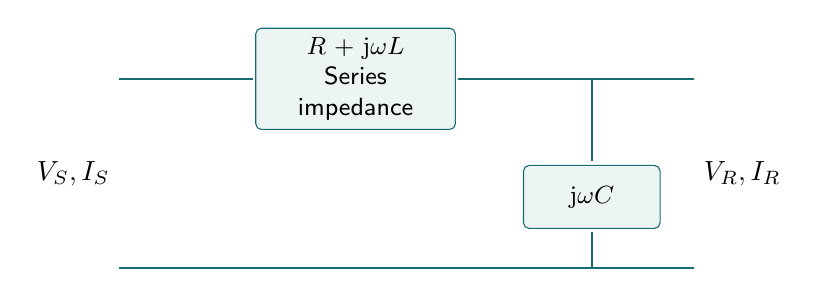
\begin{tikzpicture}
\draw[thick,teal] (0,1.4)--(1.7,1.4);
\node[block,text width=2.3cm] at (3,1.4) {$R+\jj\omega L$\\Series impedance};
\draw[thick,teal] (4.3,1.4)--(7.3,1.4);
\draw[thick,teal] (6,1.4)--(6,.35);
\node[block,text width=1.5cm,minimum height=.8cm] at (6,-.1) {$\jj\omega C$};
\draw[thick,teal] (6,-.55)--(6,-1);
\draw[thick,teal] (0,-1)--(7.3,-1);
\node[left,align=right] at (0,.2) {$V_S,I_S$};
\node[right,align=left] at (7.3,.2) {$V_R,I_R$};
\end{tikzpicture}\par\vspace{10mm}
\begin{Idea}{Built for understanding, derivation and exam preparation}
A complete explanation of the supplied Module 2 syllabus and both class slide decks: field-to-circuit derivations, labelled diagrams, every class numerical, additional examples, revision sheets and practice answers.
\end{Idea}
\vfill
{\small Comprehensive study notes covering transmission line parameters, ABCD modeling, line performance, Ferranti effect, corona, SIL, and insulator string efficiency according to the 2024-scheme syllabus.}\par\vspace{4mm}
{\small\sffamily Prepared for Sudheesh / 8 October 2026}
\end{titlepage}
\tableofcontents
\clearpage\pagenumbering{arabic}
\chapterstart{A study map for the whole module}{map}
\subsection{What the syllabus requires}
The supplied syllabus places Module 2 across PDF pp. 1--2, with 11 contact hours. Its main goal is to understand the electrical performance of transmission lines. Use the following map to track your preparation.
\begin{center}\small
\begin{tabularx}{\textwidth}{L{5.8cm}Y}
\toprule\textbf{Required topic} & \textbf{What you should be able to do}\\\midrule
Electrical model; resistance, inductance and capacitance & Explain series and shunt effects; derive internal/external flux linkage and electric potential; convert per-metre data to a complete line.\\
Three-phase double-circuit derivations & Build phase groups; compute self and mutual geometric means; derive both symmetrical and transposed vertical configurations for $L$ and $C$.\\
Transmission-line classification (concept only) & Explain why short, medium and long lines use different approximations, rather than treating a length boundary as a physical discontinuity.\\
Two-port network; ABCD derivation and numericals & Derive short-line, nominal-T and nominal-$\pi$ constants; understand distributed constants; calculate terminal quantities and check reciprocity.\\
Skin and Ferranti effects; corona (qualitative) & Explain causes, influencing factors, consequences and mitigation. Corona-loss and critical-voltage formula derivations are not demanded.\\
Surge impedance loading & Derive $Z_0=\sqrt{L'/C'}$ and three-phase $P_{\rm SIL}=V_{LL}^2/Z_0$; distinguish natural loading from a rating.\\
Insulators; string efficiency; grading numericals & Identify types, derive three/four-disc voltage distribution, apply KCL to arbitrary strings, and design ideal capacitance grading.\\\bottomrule
\end{tabularx}\end{center}
\subsection{How to use these notes}
Read Sections~\ref{foundation}--\ref{capacitance} first. Redraw each diagram and explain the reason for every term. Then work through the class parameter examples in Section~\ref{parameterexamples}. Learn the line models before attempting their performance calculations. Finish with insulator KCL, the revision sheets and the practice questions.

For every numerical, write \textbf{what the result is per}: per conductor, per phase, per circuit, per kilometre, or for the complete line. Most serious errors in this module are denominator, length or grouping errors rather than difficult arithmetic.

\begin{Caution}{Study approach and problem-solving}
These notes focus on physical derivations, clear circuit models, and error-proof problem-solving workflows. Practice questions and additional worked examples develop independent calculation skills, with emphasis on consistent per-phase, per-circuit, and per-unit bases.
\end{Caution}

\chapterstart{From a physical line to an electrical model}{foundation}
\slides{Part 1 pp. 1--9, 12, 18, 85; Part 2 pp. 1--12, 59, 79--81}
\subsection{Why a transmission line is not an ideal wire}
A real conductor dissipates energy, establishes magnetic and electric fields, and interacts with adjacent conductors and earth. The line therefore has \textbf{distributed} parameters: every small length contributes them. Their effects accumulate with length.
\begin{center}\small
\begin{tabularx}{\textwidth}{L{2.4cm}YY}
\toprule\textbf{Parameter} & \textbf{Physical meaning} & \textbf{Electrical consequence}\\\midrule
$R'$ ($\Omega$/km) & Conductor heating & Real power loss $I^2R$ and voltage drop.\\
$L'$ (H/km) & Magnetic-field energy & Series inductive reactance; reactive absorption, fault-current limitation and power-transfer constraints.\\
$C'$ (F/km) & Electric-field energy between phases and earth & Charging current even at no load; reactive supply, voltage rise and changes in surge impedance.\\
$G'$ (S/km) & Insulation/leakage path & Shunt real loss; often neglected for a clean overhead line in elementary steady-state calculations.\\\bottomrule
\end{tabularx}\end{center}
For length $\ell$ and frequency $f$, write
\[
 Z=(R'+\jj\omega L')\ell=R+\jj X,\qquad
 Y=(G'+\jj\omega C')\ell=G+\jj B_{\rm sh},\qquad \omega=2\pi f.
\]
The units of $\ell$ must match the units of the primed parameters. $B_{\rm sh}$ is susceptance; later the ABCD constant $B$ is an impedance. They share a letter but have different meanings.

The line stores $\tfrac12 LI^2$ magnetically and $\tfrac12 CV^2$ electrically for instantaneous values in ideal lumped elements. Resistance converts energy to heat; it does not store it. Inductance and capacitance exchange reactive power with the AC system. Parameter errors therefore affect voltage regulation, load flow, fault studies and protection as well as loss calculations.
\subsection{Single circuit, double circuit and a bundle}
A three-phase \textbf{single circuit} has phases $a,b,c$. A \textbf{double circuit} carries two three-phase sets, $a,b,c$ and $a',b',c'$, often on the same tower. The circuits can be operated independently; sharing a tower creates magnetic and electrostatic coupling even when they are not electrically paralleled.

In the double-circuit derivations here, corresponding phases are \textbf{connected in parallel and share current equally}: $a$ with $a'$, and similarly for $b,c$. This is an additional electrical assumption, not a consequence of the phrase ``double circuit''. An outage on a common tower can affect both circuits, so extra circuit capacity does not eliminate common-mode risks.

A \textbf{bundle} is two or more complete sub-conductors connected in parallel to form \emph{one phase}. A twin bundle on a single-circuit line is not a double-circuit line. A double-circuit line may also have bundles in each circuit.
\subsubsection{Single and double circuits}\slides{Part 1, p. 5}
\begin{center}\includegraphics[width=.94\textwidth,height=68mm,keepaspectratio]{Study_Assets/Module2/p1_005.pdf}\end{center}
\diagramcaption{Count three phase positions per circuit. The upper earth wire is a shield wire, not a fourth phase.}

\subsubsection{Single, double and multiple circuits}\slides{Part 1, p. 6}
\begin{center}\includegraphics[width=.94\textwidth,height=68mm,keepaspectratio]{Study_Assets/Module2/p1_006.pdf}\end{center}
\diagramcaption{The photographs connect the circuit count to actual tower construction.}
\subsection{Conductor construction and the slide photographs}
\textbf{Solid wire} is a single body. \textbf{Stranded wire} has many helically laid strands: it is flexible, easier to handle, and better able to accommodate vibration and mechanical loading. The helical strand length exceeds the axial line length, which slightly increases resistance.

\textbf{ACSR} means aluminium conductor steel reinforced: aluminium outer strands provide most of the conduction; a steel core provides tensile strength. \textbf{AAC} is all aluminium; \textbf{AAAC} is all aluminium alloy; composite-core/HTLS designs pursue combinations of thermal capability, strength and reduced sag. Actual conductor selection depends on conductivity, strength, weight, sag, corrosion, temperature, installation and cost. The photographs in Part 1 pp. 7--9 illustrate strand and core geometry, not a new circuit element.

``Composite conductor'' is used in two ways in the slides: a material combination such as ACSR, and an electrical group of parallel strands in the GMD derivation. State which meaning you use. In both a strand group and a bundle, an equivalent self-geometric mean accounts for the arrangement of the members.
\subsubsection{Solid and stranded conductors}\slides{Part 1, p. 7}
\begin{center}\includegraphics[width=.94\textwidth,height=68mm,keepaspectratio]{Study_Assets/Module2/p1_007.pdf}\end{center}
\diagramcaption{Stranding provides flexibility. It does not eliminate skin effect; compare with Section~\ref{resistance}.}

\subsubsection{Steel and composite cores}\slides{Part 1, p. 8}
\begin{center}\includegraphics[width=.94\textwidth,height=68mm,keepaspectratio]{Study_Assets/Module2/p1_008.pdf}\end{center}
\diagramcaption{Recognize the load-bearing core and surrounding aluminium strands. Composite cores are class context.}

\subsubsection{ACSR cross-section}\slides{Part 1, p. 9}
\begin{center}\includegraphics[width=.94\textwidth,height=68mm,keepaspectratio]{Study_Assets/Module2/p1_009.pdf}\end{center}
\diagramcaption{The steel core supplies tensile strength; aluminium carries most of the load current.}
\subsection{Phasors and three-phase quantities: the essential toolkit}
Use RMS phasors and $\jj^2=-1$. A complex number can be written
\[
 z=x+\jj y=|z|\angle\theta,\quad |z|=\sqrt{x^2+y^2},\quad
 \theta=\operatorname{atan2}(y,x).
\]
Add/subtract in rectangular form; multiply/divide in polar form or by ordinary complex algebra. Never add magnitudes of phasors with different angles.

For balanced three-phase operation,
\[
 |V_{\rm ph}|=\frac{V_{LL}}{\sqrt3},\quad
 S_{3\phi}=3V_{\rm ph}I^*=P+\jj Q,\quad
 P=\sqrt3 V_{LL}|I|\cos\phi.
\]
If $V_R$ is the reference and the load power factor is lagging, then $I_R=|I_R|\angle(-\phi)$; for leading power factor the angle is $+\phi$. Use \textbf{phase voltage} in ABCD equations. Convert its magnitude to line voltage only after the phasor calculation. The complex line-to-line voltage also has a $30^\circ$ shift relative to a phase voltage; multiplying by $\sqrt3$ here is a magnitude conversion.

For balanced currents $I_a+I_b+I_c=0$ \emph{as phasors}, even though their magnitudes are equal. Likewise balanced phase charges sum to zero instantaneously or in phasor representation; three equal magnitudes are not three identical signed charges.
\subsection{A compact unit discipline}
\begin{center}\small
\begin{tabularx}{\textwidth}{L{4.2cm}Y}
\toprule\textbf{Conversion} & \textbf{Use it for}\\\midrule
$1\ {\rm km}=10^3\ {\rm m}$ & Convert H/m or F/m to a total line value.\\
$1\ {\rm mH/km}=10^{-6}\ {\rm H/m}$ & Inductance formula outputs.\\
$1\ {\rm nF/km}=10^{-12}\ {\rm F/m}$ & Capacitance formula outputs.\\
$1\ \mu{\rm F/km}=10^{-9}\ {\rm F/m}$ & Charging-current conversion.\\
$1\ {\rm mm^2}=10^{-6}\ {\rm m^2}$ & Resistance cross-sectional area.\\
$\ln x=2.302585\log_{10}x$ & Every logarithmic formula here uses natural logarithms.\\\bottomrule
\end{tabularx}\end{center}
In $\ln(D/r)$, $D$ and $r$ can both be in metres or both in centimetres; mixing them changes the answer. The logarithm must have a dimensionless argument.

\chapterstart{Resistance and skin effect}{resistance}
\slides{Part 1 pp. 10--15; Part 2 pp. 27--31}
\subsection{DC resistance and temperature}
For a uniform conductor,
\[
 \ans{R_{\rm dc}=\rho\ell/A_c}.
\]
Here $A_c$ is the conducting area, not an ABCD constant. Typical slide reference values are $\rho_{\rm Cu}\approx1.72\times10^{-8}\ \Omega\,\mathrm m$ and $\rho_{\rm Al}\approx2.83\times10^{-8}\ \Omega\,\mathrm m$; temperature, purity and alloy affect them.

For a linear temperature approximation with coefficient referred to $T_1$,
\[
 R_{T_2}=R_{T_1}[1+\alpha_{T_1}(T_2-T_1)].
\]
If a coefficient $\alpha_0$ is specified at $0^\circ$C, then
\[
 \alpha_{T_1}=\frac{\alpha_0}{1+\alpha_0T_1},\qquad
 \frac{R_{T_2}}{R_{T_1}}=\frac{1+\alpha_0T_2}{1+\alpha_0T_1}.
\]
The slide's aluminium coefficient near $0.00403/{}^\circ$C must be used at its stated reference temperature. $75^\circ$C is a common data-reference temperature in the slide, not the operating temperature of every overhead conductor.

\textbf{Stranding correction:} the approximately 2\% slide correction is an illustration. Helical lay increases the current path; it is not a universal reduction of the actual metallic area. Use a supplied correction or manufacturer resistance/GMR data for a real stranded conductor. If modelling ACSR, do not treat the entire outer cross-sectional circle as pure aluminium without a stated approximation.
\subsection{Loss, voltage drop and parallel conductors}
For one phase, real loss is $|I|^2R$. For a balanced line with per-phase resistance $R$,
\[
 P_{\rm loss}=3|I|^2R.
\]
Heating constrains ampacity; it depends on cooling as well as electrical losses. Larger area, suitable material and temperature management reduce resistance or permit higher current.

For two \emph{identical, electrically paralleled} phase paths, $R_{\rm eq}=R_{\rm path}/2$. For $n_b$ identical sub-conductors in a phase bundle, $R_{\rm bundle}=R_{\rm sub}/n_b$. If two such circuits are paralleled,
\[
 \ans{R_{\rm eq}=\frac{R_{\rm sub}}{2n_b}}.
\]
This simple resistance result does not mean inductance halves independently of mutual coupling. Unequal paths require the parallel-resistance formula, and unequal sharing changes individual losses.
\subsection{The physical origin of skin effect}
\textbf{Skin effect} is the nonuniform distribution of AC current across a conductor: current density tends to be greater near the surface. Time-varying magnetic fields induce electric fields that oppose changes of current; inner paths have greater linked flux and effective inductive opposition than outer paths. This redistributes current and raises effective AC resistance.

The qualitative picture in the slides shows a solid DC-filled circle and progressively thinner outer AC regions. These are conceptual diagrams: at 50 Hz in an ordinary conductor, the centre need not carry zero current. Current density changes smoothly rather than stopping at a sharp ``skin'' boundary.

Skin effect grows with frequency, conductor size relative to penetration depth and magnetic permeability. It depends on resistivity too. It is absent in a steady DC state, and can be small for thin conductors at power frequency. Nearby conductors can also redistribute current by \textbf{proximity effect}, a related but different mechanism.
\subsubsection{Current penetration}\slides{Part 1, p. 14}
\begin{center}\includegraphics[width=.94\textwidth,height=68mm,keepaspectratio]{Study_Assets/Module2/p1_014.pdf}\end{center}
\diagramcaption{The darkened conducting regions are a qualitative sketch: current density varies continuously, not as a sharp hollow cylinder.}

\subsubsection{Skin-effect sections}\slides{Part 2, p. 28}
\begin{center}\includegraphics[width=.94\textwidth,height=68mm,keepaspectratio]{Study_Assets/Module2/p2_028.pdf}\end{center}
\diagramcaption{Inner filaments link more magnetic flux. The hollow-looking conducting region is a qualitative high-frequency picture.}
\subsection{Mitigation and useful qualifications}
Hollow conductors avoid using material in a poorly utilised core at sufficiently high frequency. Smaller sub-conductors can reduce skin-effect severity at a given total area. Low-permeability conducting materials help. Ordinary bare strands touch electrically: a stranded ACSR conductor is not an insulated, transposed Litz-wire winding, and stranding alone does not abolish skin effect. Real AC resistance includes conductor geometry, skin/proximity effects and, for ACSR, possible magnetic-core effects.

As an optional physical scale, the good-conductor skin-depth estimate is
\[
 \delta\approx\sqrt{\frac{2\rho}{\omega\mu}}.
\]
Using the slide's copper resistivity, $f=50$ Hz and $\mu=\mu_0$ gives about \textbf{9.3 mm}. The slide phrase ``a few millimetres'' is not an accurate universal 50-Hz copper value. This estimate is not a sharp boundary or a full AC-resistance calculation for a small round wire.
\checkq{Does a bundle reduce the resistance, inductance and corona in the same way?}{Resistance falls by parallel paths; inductance changes through self/mutual magnetic geometry; corona is reduced through a lower surface electric field. They are distinct mechanisms.}

\chapterstart{Inductance from flux linkage}{inductance}
\slides{Part 1 pp. 16--39, 53--57}
\subsection{Flux linkage and the assumptions}
Flux linkage $\lambda$ is measured in Wb-turn; inductance is $L=\lambda/I$ for a linear magnetic system. Per-length flux linkage gives H/m. For overhead line conductor derivations assume long parallel conductors, circular cross sections, air outside, balanced return currents and low-frequency uniform current density when including the simple internal term. For a nonmagnetic solid round conductor, $\mu\approx\mu_0=4\pi\times10^{-7}$ H/m.

A distributed conductor is not literally a single discrete coil. The class relation $N\Phi$ helps introduce flux linkage, but internal flux must be weighted by the fraction of current it links. That weighting produces the $1/4$ term below.
\subsubsection{Magnetic loops}\slides{Part 1, p. 19}
\begin{center}\includegraphics[width=.94\textwidth,height=68mm,keepaspectratio]{Study_Assets/Module2/p1_019.pdf}\end{center}
\diagramcaption{Circular flux paths around a long conductor explain the Ampere-law integration.}

\subsubsection{Internal and external flux}\slides{Part 1, p. 20}
\begin{center}\includegraphics[width=.94\textwidth,height=68mm,keepaspectratio]{Study_Assets/Module2/p1_020.pdf}\end{center}
\diagramcaption{Internal flux links only a fraction of the total current; external flux links all the conductor current.}
\subsection{Derive internal flux linkage step by step}
For conductor radius $r$ and uniform current $I$, consider radius $x<r$ and a shell $dx$. The enclosed current is
\[
 I_x=I\frac{\pi x^2}{\pi r^2}=I\frac{x^2}{r^2}.
\]
Ampere's law gives $H_x(2\pi x)=I_x$, hence
\[
 H_x=\frac{Ix}{2\pi r^2},\qquad B_x=\frac{\mu Ix}{2\pi r^2}.
\]
For one metre of length, the flux in the shell is $d\Phi=B_x dx$. Only fraction $I_x/I=x^2/r^2$ links it, so
\[
 d\lambda_{\rm int}=\frac{x^2}{r^2}d\Phi
 =\frac{\mu I x^3}{2\pi r^4}\,dx.
\]
Integrate from the centre to the surface:
\[
 \lambda_{\rm int}=\frac{\mu I}{2\pi r^4}\int_0^r x^3dx
 =\frac{\mu I}{8\pi},\qquad
 \ans{L'_{\rm int}=\frac{\mu}{8\pi}}.
\]
For $\mu=\mu_0$, $L'_{\rm int}=5\times10^{-8}$ H/m $=0.05$ mH/km. It is independent of radius \emph{under uniform current density}; skin effect changes the internal contribution.
\subsubsection{Internal cylindrical shell}\slides{Part 1, p. 22}
\begin{center}\includegraphics[width=.94\textwidth,height=68mm,keepaspectratio]{Study_Assets/Module2/p1_022.pdf}\end{center}
\diagramcaption{Identify shell radius x, thickness dx and the fraction of current enclosed.}
\subsection{Derive external linkage and equivalent radius}
Outside the conductor, all the current is enclosed. At distance $x>r$,
\[
 H_x=\frac{I}{2\pi x},\quad B_x=\frac{\mu_0I}{2\pi x},\quad
 d\lambda_{\rm ext}=d\Phi=\frac{\mu_0I}{2\pi x}dx.
\]
Between radii $d_1$ and $d_2$,
\[
 \lambda_{\rm ext}=\frac{\mu_0 I}{2\pi}\ln\frac{d_2}{d_1}.
\]
For the usual two-wire return-path approximation with spacing $D\gg r$, one conductor has
\[
 L'=\frac{\mu_0}{2\pi}\left[\ln\frac Dr+\frac14\right]
 =2\times10^{-7}\ln\frac D{r'}\quad\mathrm{H/m},
 \qquad \ans{r'=re^{-1/4}=0.7788r}.
\]
$r'$ is the \textbf{geometric mean radius (GMR)}, also called self-GMD. It incorporates internal magnetic linkage. It is not a physical hollowing of the wire. Use a tabulated GMR for a stranded/composite conductor; $0.7788r$ is the solid nonmagnetic formula.

For two identical nonmagnetic conductors,
\[
 \ans{L'_{\rm loop}=4\times10^{-7}\ln(D/r')}\ \mathrm{H/m},\qquad
 L_{\rm loop}=0.4\ln(D/r')\ \mathrm{mH/km}.
\]
For magnetic material with an assumed uniform current distribution and relative permeability $\mu_r$,
\[
 L_{\rm loop}=\left[0.1\mu_r+0.4\ln(D/r)\right]\ \mathrm{mH/km}.
\]
Do not combine $0.7788r$ with this separate internal term; that would count internal flux twice. The high-$\mu_r$ steel examples are idealised class calculations, not realistic AC magnetic-loss models.
\subsubsection{External cylindrical shell}\slides{Part 1, p. 24}
\begin{center}\includegraphics[width=.94\textwidth,height=68mm,keepaspectratio]{Study_Assets/Module2/p1_024.pdf}\end{center}
\diagramcaption{Integrate the external field between the conductor surface and the return-path distance.}
\subsection{Flux linkage of a conductor among many conductors}
Use superposition. Introduce a distant reference radius $R_0$:
\[
 \lambda_i=\frac{\mu_0}{2\pi}
 \left[I_i\ln\frac{R_0}{r_i'}+\sum_{j\ne i}I_j\ln\frac{R_0}{D_{ij}}\right].
\]
When $\sum_j I_j=0$, the arbitrary $\ln R_0$ terms cancel. The result depends only on conductor distances and self-GMR. The slide shorthand $\sum I_j\ln(1/D_{ij})$ is understood through that cancellation; taking a logarithm of a dimensional distance by itself is not a complete physical definition.
\subsubsection{Flux linkage with a reference point}\slides{Part 1, p. 30}
\begin{center}\includegraphics[width=.94\textwidth,height=68mm,keepaspectratio]{Study_Assets/Module2/p1_030.pdf}\end{center}
\diagramcaption{Each other conductor contributes a logarithmic distance term; the sum of balanced currents removes the remote reference.}
\subsection{Composite groups: derive self and mutual GMD}
Suppose group $A$ has $m$ parallel conductors carrying total $I_A$, each carrying $I_A/m$, and group $B$ has $n$ conductors carrying $-I_A$, each carrying $-I_A/n$. Average the linkages of the $m$ members and divide by the \emph{total group current}. Products appear because the average of logarithms is the logarithm of a geometric mean:
\[
 \frac1N\sum_{k=1}^{N}\ln d_k=\ln\left(\prod_{k=1}^{N}d_k\right)^{1/N}.
\]
Define
\[
 D_{sA}=\left(\prod_{i=1}^{m}\prod_{j=1}^{m}D^{(L)}_{ij}\right)^{1/m^2},
 \quad D^{(L)}_{ii}=r_i',\qquad
 D_{AB}=\left(\prod_{i\in A}\prod_{j\in B}D_{ij}\right)^{1/(mn)}.
\]
The group inductance becomes
\[
 \ans{L_A'=2\times10^{-7}\ln(D_{AB}/D_{sA})}.
\]
Group $B$ similarly uses its own $D_{sB}$; loop inductance is $L_A'+L_B'$. If the groups have identical self-GMD, the loop coefficient is $4\times10^{-7}$. Self products contain \textbf{ordered pairs}: $D_{ij}$ and $D_{ji}$ both occur, while the diagonal uses GMR rather than a zero distance.
\subsubsection{Composite conductor groups}\slides{Part 1, p. 34}
\begin{center}\includegraphics[width=.94\textwidth,height=68mm,keepaspectratio]{Study_Assets/Module2/p1_034.pdf}\end{center}
\diagramcaption{Use every cross-group pair for mutual GMD and all ordered within-group pairs for self GMD.}
\subsection{Three phases and transposition}
For balanced current and equal phase spacing $D$, all mutual-distance logarithms are equal. Since $I_b+I_c=-I_a$,
\[
 \lambda_a=2\times10^{-7}I_a\ln(D/r'),\qquad L_a'=2\times10^{-7}\ln(D/r').
\]
Unequal spacings yield unequal effective phase linkage/impedance. \textbf{Transposition} exchanges the phase positions over three equal sections, so each phase occupies each position for one third of the length. Average \emph{logarithmic linkage terms}, not the spacings arithmetically:
\[
 \ans{D_m=(D_{ab}D_{bc}D_{ca})^{1/3}},\qquad
 \ans{L'_{\rm ph}=2\times10^{-7}\ln(D_m/r')}.
\]
\begin{center}
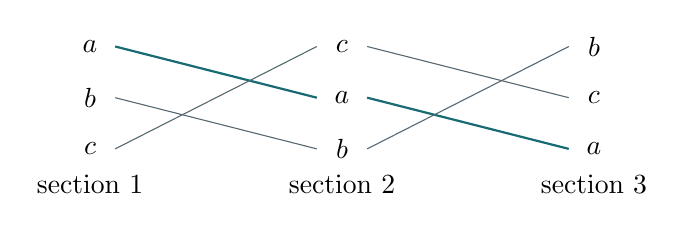
\begin{tikzpicture}[x=1.6cm,y=.65cm]
\foreach \x/\a/\b/\c in {0/a/b/c,2/c/a/b,4/b/c/a}{
 \node at (\x,2){$\a$};\node at (\x,1){$\b$};\node at (\x,0){$\c$};}
\draw[teal,thick] (.2,2)--(1.8,1);\draw[teal,thick] (2.2,1)--(3.8,0);
\draw[muted] (.2,1)--(1.8,0);\draw[muted] (2.2,0)--(3.8,2);
\draw[muted] (.2,0)--(1.8,2);\draw[muted] (2.2,2)--(3.8,1);
\node at (0,-.7){section 1};\node at (2,-.7){section 2};\node at (4,-.7){section 3};
\end{tikzpicture}
\end{center}
\diagramcaption{The teal path tracks phase $a$. Each section is $\ell/3$. This is a position map, not a picture of conductors touching.}
A double-circuit three-section transposition does not make one conductor visit all six physical sites. It cycles each member through the positions specified in its transposition scheme; corresponding phase-group geometry must be averaged consistently. Without suitable transposition/balance, use the full coupled impedance matrix rather than a single scalar $L$.
\subsubsection{Three-phase transposition}\slides{Part 1, p. 39}
\begin{center}\includegraphics[width=.94\textwidth,height=68mm,keepaspectratio]{Study_Assets/Module2/p1_039.pdf}\end{center}
\diagramcaption{Each phase occupies each physical position for one third of a full transposition cycle.}
\subsection{Bundles: two, three and four sub-conductors}
For equal current sharing, sub-conductor GMR $r'$ and adjacent spacing $s$, the self-product formula gives
\begin{center}\small
\begin{tabularx}{\textwidth}{L{4.2cm}YY}
\toprule\textbf{Bundle geometry} & \textbf{Magnetic self-GMD} & \textbf{Why}\\\midrule
Twin & $D_s=\sqrt{r's}$ & One self term and one neighbour per row.\\
Equilateral triplex & $D_s=(r's^2)^{1/3}$ & Two neighbours, both at $s$.\\
Square quad & $D_s=(r'\sqrt2\,s^3)^{1/4}$ & Two neighbours at $s$, one diagonal at $\sqrt2s$.\\\bottomrule
\end{tabularx}\end{center}
The square factor is $2^{1/8}\approx1.0905$. Specify square side spacing; a different geometry needs different distances. If phase spacing is much greater than $s$, bundle centres give a good approximate $D_m$. Exact mutual GMD uses all pair distances. Then $L'_{\rm ph}=2\times10^{-7}\ln(D_m/D_s)$ \emph{already includes parallel current sharing}. Do not divide it by the number of sub-conductors again.

Increasing effective self-GMD lowers $L$ and $X$; it also lowers electric surface stress and changes $C$ and SIL. Spacers preserve bundle geometry and resist clashing/vibration. The statements about higher transfer capability depend on the rest of the system, not only this one parameter.
\subsubsection{Hexagon and tower arrangements}\slides{Part 1, p. 41}
\begin{center}\includegraphics[width=.94\textwidth,height=68mm,keepaspectratio]{Study_Assets/Module2/p1_041.pdf}\end{center}
\diagramcaption{The geometrical conductor diagram is the electrical model; the tower is its physical support.}

\subsubsection{Bundle spacers and suspension}\slides{Part 1, p. 53}
\begin{center}\includegraphics[width=.94\textwidth,height=68mm,keepaspectratio]{Study_Assets/Module2/p1_053.pdf}\end{center}
\diagramcaption{Subconductors of a bundle belong to one phase. The spacer fixes bundle geometry; circuit count is a separate idea.}
\chapterstart{Three-phase double-circuit inductance}{doubleL}
\slides{Part 1 pp. 40--52, 76--79, 82}
\subsection{Define the current before deriving anything}
Let \textbf{total phase current} be $I_A$ and each parallel member carry $i_A=I_A/2$. The other phase groups carry $I_B,I_C$, with $I_A+I_B+I_C=0$. Assume corresponding phases have equal voltage and symmetric/equal sharing, and neglect earth-return effects for balanced positive-sequence operation.

For group $A=\{a,a'\}$ with identical member GMR $r'$, its magnetic self-GMD is
\[
 D_{sA}=(r'D_{aa'}D_{a'a}r')^{1/4}=\sqrt{r'D_{aa'}}.
\]
Between groups $A,B$,
\[
 D_{AB}=(D_{ab}D_{ab'}D_{a'b}D_{a'b'})^{1/4}.
\]
Compute the other two self and mutual groups similarly. Under the appropriate complete transposition,
\[
 D_s=(D_{sA}D_{sB}D_{sC})^{1/3},\qquad
 D_m=(D_{AB}D_{BC}D_{CA})^{1/3}.
\]
\begin{Idea}{The general double-circuit result}
\[
 \ans{L'_{\rm eq,ph}=2\times10^{-7}\ln(D_m/D_s)}\quad\mathrm{H/m}.
\]
This is for a phase group carrying the \emph{sum} of its two conductor currents. The self-GMD already incorporates sharing, so no further factor of $1/2$ is applied. It is the safest form for a numerical with an arbitrary drawn tower geometry.
\end{Idea}
\subsection{Derive the symmetrical regular-hexagon case}
Place six conductors at a regular hexagon of side $d$ in cyclic order $a,c',b',a',c,b$. Corresponding phases are opposite, separated by $2d$. Cross-phase distances alternate $d$ and $\sqrt3d$.
\begin{center}
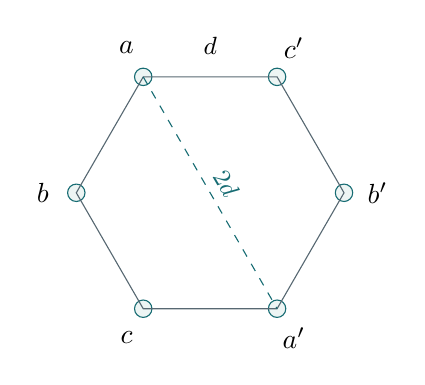
\begin{tikzpicture}[scale=.85]
\foreach \ang/\name in {120/a,60/c',0/b',300/a',240/c,180/b}{
 \draw[fill=pale,draw=teal] (\ang:2) circle (.13);\node at (\ang:2.5){$\name$};}
\draw[muted] (120:2)--(60:2)--(0:2)--(300:2)--(240:2)--(180:2)--cycle;
\draw[dashed,teal] (120:2)--node[above,sloped]{\small $2d$}(300:2);
\node at (0,2.2){\small $d$};
\end{tikzpicture}
\end{center}
Thus
\[
 D_s=\sqrt{2dr'},\qquad
 D_{AB}=D_{BC}=D_{CA}=(d\,\sqrt3d\,\sqrt3d\,d)^{1/4}=3^{1/4}d.
\]
Substitute into the group result:
\[
 \begin{aligned}
 L'_{\rm eq,ph}
 &=2\times10^{-7}\ln\frac{3^{1/4}d}{\sqrt{2dr'}}\\
 &=\ans{10^{-7}\ln\frac{\sqrt3d}{2r'}}\quad\mathrm{H/m}.
 \end{aligned}
\]
To connect with the class conductor-by-conductor derivation, the linkage of member $a$ is
\[
 \lambda_a=2\times10^{-7}\left[
 i_A\ln\frac1{r'}+i_A\ln\frac1{2d}
 +(i_B+i_C)\ln\frac1{\sqrt3d^2}\right].
\]
Because $i_B+i_C=-i_A$, this is $2\times10^{-7}i_A\ln[\sqrt3d/(2r')]$. Dividing by member current gives a member-effective coefficient. Dividing by \emph{total} current $I_A=2i_A$ gives the phase-group result above. The ``divide by two'' in Part 1 pp. 43--44 is correct in this particular member-current derivation; it is not an extra step after the general group formula.
\subsubsection{All three double-circuit positions}\slides{Part 1, p. 45}
\begin{center}\includegraphics[width=.94\textwidth,height=68mm,keepaspectratio]{Study_Assets/Module2/p1_045.pdf}\end{center}
\diagramcaption{Track phase partners through all three positions. Take the geometric mean of their group quantities; do not average distances arithmetically.}
\subsection{Derive the transposed vertical configuration}
Consider the specific arrangement used in Part 1 p. 45. Left column top to bottom: $a,b,c$; right column: $c',b',a'$. Vertical adjacent spacing is $d_1$; horizontal separation is $d_2$. Let
\[
 F=\sqrt{4d_1^2+d_2^2},\qquad E=\sqrt{d_1^2+d_2^2}.
\]
\begin{center}
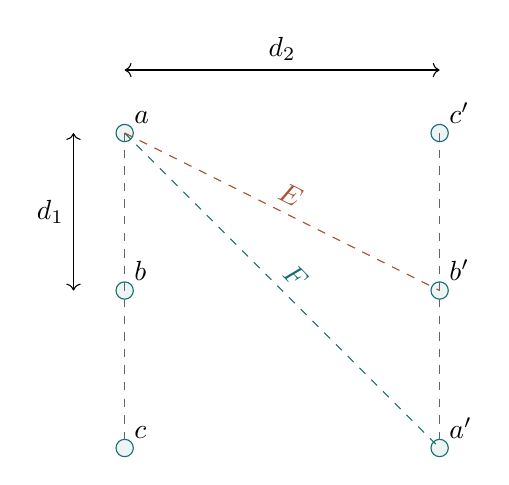
\begin{tikzpicture}[x=1cm,y=1cm]
\foreach \x/\y/\name in {0/2/a,0/0/b,0/-2/c,4/2/c',4/0/b',4/-2/a'}{
 \draw[fill=pale,draw=teal] (\x,\y) circle(.11);\node[above right] at (\x,\y){$\name$};}
\draw[muted,dashed] (0,2)--(0,-2);\draw[muted,dashed] (4,2)--(4,-2);
\draw[<->] (-.65,0)--node[left]{$d_1$}(-.65,2);
\draw[<->] (0,2.8)--node[above]{$d_2$}(4,2.8);
\draw[dashed,teal] (0,2)--node[above,sloped]{$F$}(4,-2);
\draw[dashed,rust] (0,2)--node[above,sloped]{$E$}(4,0);
\end{tikzpicture}
\end{center}
The phase-group self distances are
\[
 D_{sA}=D_{sC}=\sqrt{r'F},\quad D_{sB}=\sqrt{r'd_2},\quad
 D_s=r'^{1/2}F^{1/3}d_2^{1/6}.
\]
The mutual distances are
\[
 D_{AB}=D_{BC}=(d_1^2E^2)^{1/4},\quad
 D_{CA}=[(2d_1)^2d_2^2]^{1/4}.
\]
After averaging over the equal transposition sections,
\[
 D_m=2^{1/6}d_1^{1/2}d_2^{1/6}(d_1^2+d_2^2)^{1/6}.
\]
The common $d_2^{1/6}$ cancels in $D_m/D_s$, giving
\[
 \ans{L'_{\rm eq,ph}=2\times10^{-7}\ln\left[
 2^{1/6}\left(\frac{d_1}{r'}\right)^{1/2}
 \left(\frac{d_1^2+d_2^2}{4d_1^2+d_2^2}\right)^{1/6}\right]}.
\]
The result is H/m. This derives the full expression in Part 1 pp. 48, 51--52 while preserving the units of the actual self and mutual GMDs. The shortened numerator/denominator on p. 48 omit the same cancelling $d_2^{1/6}$; their ratio works, but separately they are not geometric distances measured in metres.

If $d_2\gg d_1$, the last ratio tends to one and
\[
 L'_{\rm eq,ph}\approx2\times10^{-7}\ln\left[2^{1/6}(d_1/r')^{1/2}\right].
\]
That simplification is tied to this phase arrangement. If the right-hand column has a different phase order, recompute its distances. Do not apply this closed form to an arbitrary six-conductor tower.
\subsection{Why coupling prevents a blind \texorpdfstring{$L/2$}{L/2} rule}
For two identical coupled paths with self $L_s$ and mutual $M$, equal sharing gives $L_{\rm eq}=(L_s+M)/2$, not generally $L_s/2$. The group-GMD method builds the relevant mutual linkage into the geometry. Independent circuits, untransposed layouts or unequal currents need a coupled model. The slide claims ``lower inductance, higher capacitance and higher SIL'' describe an appropriate combined arrangement relative to a chosen single-circuit comparison, not every possible arrangement.
\checkq{A double-circuit answer was found with $D_s=\sqrt{r'D_{aa'}}$. Should it be divided by two again?}{No. This self-GMD and the $2\times10^{-7}$ group formula use total phase current. A second division double-counts parallel sharing.}

\chapterstart{Capacitance from electric field and potential}{capacitance}
\slides{Part 1 pp. 83--106, 111--118}
\subsection{Gauss's law and the radial electric field}
Let a long conductor carry charge per length $q$ C/m. A cylindrical Gaussian surface of radius $x$ and length $\ell$ encloses $q\ell$. Gauss's law gives
\[
 E_x(2\pi x\ell)=q\ell/\varepsilon,\qquad
 \ans{E_x=\frac{q}{2\pi\varepsilon x}}.
\]
For air, $\varepsilon\approx\varepsilon_0=8.854\times10^{-12}$ F/m. For two radial locations $x_1<x_2$, the inner point is at higher potential for positive charge:
\[
 V(x_1)-V(x_2)=\int_{x_1}^{x_2}E_xdx
 =\frac{q}{2\pi\varepsilon}\ln\frac{x_2}{x_1}.
\]
Capacitance is charge divided by the relevant potential difference: $C'=q/V$.

\begin{Caution}{Do not assign an isolated infinite line a finite potential at infinity}
For one infinite charged conductor, $\int_r^\infty dx/x$ diverges. Part 1 p. 91 is a formal intermediate, not a finite self-potential. Use a finite reference, a return conductor/earth, or a charge-neutral collection. When $\sum q_i=0$, arbitrary distant-reference terms cancel in potential differences, just as the remote reference cancels in balanced magnetic linkage.
\end{Caution}
\subsubsection{Radial electric field}\slides{Part 1, p. 84}
\begin{center}\includegraphics[width=.94\textwidth,height=68mm,keepaspectratio]{Study_Assets/Module2/p1_084.pdf}\end{center}
\diagramcaption{Gauss law gives E proportional to 1/x outside a long round conductor. Potential is the integral of this field.}

\subsubsection{Phase and earth capacitance}\slides{Part 1, p. 86}
\begin{center}\includegraphics[width=.94\textwidth,height=68mm,keepaspectratio]{Study_Assets/Module2/p1_086.pdf}\end{center}
\diagramcaption{This is a conceptual sketch. Use the balanced per-phase model and image-conductor derivation in Section~\ref{capacitance} for calculations.}

\subsubsection{Potential between radii}\slides{Part 1, p. 91}
\begin{center}\includegraphics[width=.94\textwidth,height=68mm,keepaspectratio]{Study_Assets/Module2/p1_091.pdf}\end{center}
\diagramcaption{Only potential differences are finite for an isolated infinite line charge. Do not set its potential at infinity to zero.}
\subsection{Single-phase two-wire capacitance: the factor of two}
For two identical wires of radius $r$, separation $D\gg r$, charges $+q$ and $-q$, neglecting earth,
\[
 V_{ab}=\frac q{\pi\varepsilon}\ln\frac Dr,
 \quad \ans{C'_{ab}=\frac{\pi\varepsilon}{\ln(D/r)}}.
\]
The neutral lies midway in potential, so $V_{an}=V_{ab}/2$ and
\[
 \ans{C'_n=\frac{2\pi\varepsilon}{\ln(D/r)}=2C'_{ab}}.
\]
The two equal phase-to-neutral capacitances in series give $C_{ab}$. ``Line-to-earth'' in Part 1 p. 94 means the elementary equivalent neutral reference in this calculation; actual nearby-earth capacitance requires the image method. Always say whether the question asks for \emph{between-wire capacitance} or \emph{capacitance to neutral}.
\subsubsection{Two-wire charges}\slides{Part 1, p. 95}
\begin{center}\includegraphics[width=.94\textwidth,height=68mm,keepaspectratio]{Study_Assets/Module2/p1_095.pdf}\end{center}
\diagramcaption{Opposite charges set the phase-to-phase voltage; the capacitance to neutral is twice the two-wire capacitance.}
\subsection{Three-phase single circuit, including transposition}
Introduce a common distant reference $R_0$. The phase-$a$ potential is
\[
 V_{an}=\frac1{2\pi\varepsilon}
 \left[q_a\ln\frac{R_0}{r}+q_b\ln\frac{R_0}{D_{ab}}
 +q_c\ln\frac{R_0}{D_{ac}}\right].
\]
Under balanced charge, $q_a+q_b+q_c=0$, so the reference cancels. In equilateral spacing, $D_{ab}=D_{ac}=D$, yielding
\[
 V_{an}=\frac{q_a}{2\pi\varepsilon}\ln(D/r),\qquad
 C'_n=\frac{2\pi\varepsilon}{\ln(D/r)}.
\]
For unequal spacings, averaging three equal transposition sections replaces the distance by $D_m=(D_{ab}D_{bc}D_{ca})^{1/3}$. Thus
\[
 \ans{C'_n=\frac{2\pi\varepsilon}{\ln(D_m/r)}}.
\]
For an untransposed asymmetric line, solve the coupled potential equations for charges at the imposed phase voltages; three independent identical scalar capacitances need not represent it. The expanded expressions in Part 1 pp. 96--98 express this coupling. Transposition is the simplification that produces the scalar formula above.

\textbf{Use physical radius $r$, not $0.7788r$.} There is no internal electric-field term corresponding to internal magnetic flux in an ideal conducting body. Increasing radius raises capacitance; increasing phase separation lowers it.
\subsubsection{Superposition of line charges}\slides{Part 1, p. 92}
\begin{center}\includegraphics[width=.94\textwidth,height=68mm,keepaspectratio]{Study_Assets/Module2/p1_092.pdf}\end{center}
\diagramcaption{Sum the potential contributions of all charges before using balanced-charge cancellation.}
\subsection{Double circuit: derive the correct equivalent capacitance}
Assume equal member charges $q_a=q_{a'}=q_A/2$ and corresponding phases connected in parallel. Use the same phase-group averaging as for inductance, but replace each self-diagonal GMR $r'$ by \textbf{physical radius $r$}. Define
\[
 D^{(C)}_{sA}=\sqrt{rD_{aa'}},\qquad
 D^{(C)}_s=(D^{(C)}_{sA}D^{(C)}_{sB}D^{(C)}_{sC})^{1/3}.
\]
Mutual $D_m$ depends only on geometry, so it is unchanged. Averaging member potentials gives
\[
 V_{An}=\frac{q_A}{2\pi\varepsilon}\ln\frac{D_m}{D^{(C)}_s},\qquad
 \ans{C'_{\rm eq,ph}=\frac{2\pi\varepsilon}{\ln(D_m/D^{(C)}_s)}}.
\]
This is \textbf{already the combined phase-group capacitance}. If $q_a$ is used instead of total charge $q_A$, $q_a/V_{An}$ is half this result. That is where the conductor-to-phase multiplication by two in the detailed slides comes from.

For the regular hexagon,
\[
 \ln\frac{D_m}{D_s^{(C)}}=\frac12\ln\frac{\sqrt3d}{2r},\qquad
 \ans{C'_{\rm eq,ph}=\frac{4\pi\varepsilon}{\ln[\sqrt3d/(2r)]}}.
\]
For the transposed vertical arrangement,
\[
 \ans{C'_{\rm eq,ph}=\frac{2\pi\varepsilon}{
 \ln\left[2^{1/6}(d_1/r)^{1/2}
 \left(\frac{d_1^2+d_2^2}{4d_1^2+d_2^2}\right)^{1/6}\right]}}.
\]
Equivalently, double the logarithm inside the expression and use numerator $4\pi\varepsilon$, as in Part 1 p. 105. Do not double the combined group result again. Part 1 p. 88 is an abbreviated summary that obscures the distinction between physical radius and magnetic GMR, and between member and total phase charge; the detailed derivation resolves both.
\subsection{Bundled-conductor capacitance}
If equal charges share a bundle, the electric self-geometric radius $r_b$ uses physical $r$:
\[
 r_b=\sqrt{rs}\ \text{(twin)},\quad
 r_b=(rs^2)^{1/3}\ \text{(equilateral triplex)},\quad
 r_b=(\sqrt2rs^3)^{1/4}\ \text{(square quad)}.
\]
Then $C'_n=2\pi\varepsilon/\ln(D_m/r_b)$. Compare with magnetic $D_s$ using $r'$. Both formulas include all members of the bundle; neither needs an extra bundle multiplier afterwards.
\subsection{Charging current and reactive power}
For total phase-to-neutral capacitance $C_n=C'_n\ell$,
\[
 I_c=\jj\omega C_nV_{\rm ph},\qquad |I_c|=\omega C_n|V_{\rm ph}|.
\]
It leads voltage by $90^\circ$. Charging-current magnitude is not load current, and continues at open circuit. With voltage approximately uniform, capacitive reactive supply magnitude is
\[
 Q_c\approx3\omega C_nV_{\rm ph}^2=\omega C_nV_{LL}^2.
\]
Use $V_{LL}$ in volts to get var. A typical $C'=10$ nF/km at 220 kV and 50 Hz gives about $0.40$ A per kilometre per phase, not ``tens of amperes per kilometre'' as suggested in Part 1 p. 87. A long complete line can have tens of amperes of charging current.
\subsection{Effect of earth: the image method}
Replace a perfectly conducting flat earth plane by negative image charges below it. A conductor at height $h_i$ has image at $-h_i$. For a collection of conductors,
\[
 V_i=\frac1{2\pi\varepsilon}
 \left[q_i\ln\frac{2h_i}{r_i}+
 \sum_{j\ne i}q_j\ln\frac{H_{ij}}{D_{ij}}\right],
\]
where $H_{ij}$ is distance from real conductor $i$ to image of conductor $j$. Solve these potential equations for charge at known voltages. This matrix formulation handles balanced and unbalanced cases without inventing a universal percentage correction.
\begin{center}
\begin{tikzpicture}[x=1cm,y=.7cm]
\draw[thick,muted] (-1,0)--(5,0);\node[right] at (5,0){earth: $V=0$};
\foreach \x/\name in {0/a,4/b}{
 \draw[fill=pale,teal] (\x,2) circle(.12);\node[above] at (\x,2){$+q_\name$};
 \draw[dashed,rust] (\x,-2) circle(.12);\node[below] at (\x,-2){$-q_\name$};}
\draw[dashed,rust] (0,2)--node[above,sloped]{$H_{ab}$}(4,-2);
\draw[<->] (-.6,0)--node[left]{$h$}(-.6,2);
\end{tikzpicture}
\end{center}
For a two-wire pair at equal height $h$, separation $D$, charges $\pm q$,
\[
 C'_n=\frac{2\pi\varepsilon}{\ln\left[\frac{2hD}{r\sqrt{D^2+4h^2}}\right]}.
\]
Since $2h/\sqrt{D^2+4h^2}<1$, the denominator is slightly smaller than $\ln(D/r)$: \textbf{earth increases the capacitance in this example}. For very large $h/D$, the correction tends to zero. Part 1 p. 89's blanket statement that earth reduces capacitance is not the result of this image calculation. Earth effects are especially important when charge balance is absent; the scalar balanced formula is an approximation, not a universal substitute for the matrix.
\chapterstart{All class numericals: line parameters}{parameterexamples}
The 18 examples below cover every numerical in Part 1. Their original example numbers have gaps; no missing number has been invented. Calculations use natural logarithms and retain precision until the final answer. Small differences from printed answers generally result from intermediate rounding; substantial discrepancies are explained.
\subsection{Example 5.1: single-phase loop inductance and reactance}
\slides{Part 1 pp. 58--59}
Two wires have diameter $1.25$ cm, spacing 1 m, frequency 50 Hz. Find loop inductance and reactance per kilometre.
\[
 r=0.00625\ \mathrm m,\quad r'=0.7788r=0.0048675\ \mathrm m,
 \quad L_{\rm loop}=0.4\ln\frac1{0.0048675}=\ans{2.130\ \mathrm{mH/km}}.
\]
\[
 X_{\rm loop}=2\pi(50)(2.130\times10^{-3})=\ans{0.6692\ \Omega/\mathrm{km}}.
\]
One conductor's inductance is half the loop value. The question asks for the complete outgoing-and-return loop.
\subsection{Example 5.2: area instead of diameter}
\slides{Part 1 pp. 60--61}
A 500 m single-phase two-wire line has area 10 cm$^2$ per wire and spacing 5 m.
\[
 r=\sqrt{10/\pi}\ \mathrm{cm}=1.7841\ \mathrm{cm},\quad
 r'=1.3895\ \mathrm{cm}=0.013895\ \mathrm m.
\]
\[
 L_{\rm loop,500m}=0.4\ln\frac5{0.013895}\,(0.5)
 =\ans{1.1771\ \mathrm{mH}}.
\]
$0.5$ is the length in kilometres. The result is for the entire 500 m line, not mH/km.
\subsection{Example 5.3: copper versus idealised steel}
\slides{Part 1 pp. 62--63}
Two wires are 1 m apart, each diameter 1 cm. Compare copper ($\mu_r=1$) and steel ($\mu_r=50$) loop inductance per kilometre under uniform current density.
\[
 r=0.005\ \mathrm m,\qquad L_{\rm loop}=0.1\mu_r+0.4\ln\frac1{0.005}.
\]
\[
 \ans{L_{\rm Cu}=2.2193\ \mathrm{mH/km}},\qquad
 \ans{L_{\rm steel}=7.1193\ \mathrm{mH/km}}.
\]
The external term is the same; the difference $0.1(50-1)=4.9$ mH/km is the idealised internal magnetic contribution. Real steel permeability, AC current distribution and magnetic losses require a more detailed model.
\subsection{Example 5.4: high-permeability steel}
\slides{Part 1 pp. 64--65}
Diameter 1.2 cm, separation 2.5 m, relative permeability 200:
\[
 L_{\rm loop}=0.1(200)+0.4\ln\frac{2.5}{0.006}
 =\ans{22.413\ \mathrm{mH/km}}.
\]
Use physical radius in the external term and add the separate $\mu_r$ term. Using $0.7788r$ here would mix two internal-flux conventions.
\subsection{Example 5.5: the seven-strand GMR model}
\slides{Part 1 pp. 66--67}
The source asks about a six-aluminium/one-steel strand ACSR construction. Its solution explicitly takes \textbf{strand radius} $r=3$ mm, and assigns each strand the same self-GMR $0.7788r$ and equal current. Reproduce that idealised geometric calculation before applying it to a real conductor.

Six touching outer strand centres form a hexagon around a central strand. In one outer row, the six mutual distances are $2r,2\sqrt3r,4r,2\sqrt3r,2r,2r$; the diagonal is $0.7788r$. The row product is $299.0592r^7$. The centre row has product $0.7788(2^6)r^7=49.8432r^7$. There are six outer rows and one centre row, so
\[
 D_s=\left[(299.0592r^7)^6(49.8432r^7)\right]^{1/49}
 =2.1767r=\ans{6.530\ \mathrm{mm}}.
\]
The slide rounds to 6.528 mm. If ``3 mm'' is specified as a \emph{diameter}, the strand radius is 1.5 mm and this same model gives about 3.265 mm. Do not silently mix the two interpretations. Actual ACSR has unequal material properties and current sharing; obtain its GMR from manufacturer data rather than declaring the idealised seven-equal-strand result exact.
\subsection{Example 5.6: two conductors in each single-phase path}
\slides{Part 1 pp. 68--69}
The outgoing pair occupies positions $x=0,0.2$ m; the return pair $x=1.4,1.6$ m. Every wire has radius 1.2 cm; current shares equally in each pair.
\[
 r'=0.7788(0.012)=0.0093456\ \mathrm m,\qquad
 D_s=\sqrt{0.0093456(0.2)}=0.043233\ \mathrm m.
\]
The four cross-path distances are $1.4,1.6,1.2,1.4$ m:
\[
 D_m=(1.4\times1.6\times1.2\times1.4)^{1/4}=1.39280\ \mathrm m.
\]
\[
 L_{\rm loop}=0.4\ln(D_m/D_s)=\ans{1.38898\ \mathrm{mH/km}}.
\]
The diagram's 1.2 m is the \emph{gap between inner wires}, not centre-to-centre group separation. Correct distance interpretation matters more than a remembered bundle formula.
\subsection{Example 5.8: equilateral three-phase line}
\slides{Part 1 pp. 70--71}
Diameter 1.24 cm, equilateral side 2 m:
\[
 r=0.0062\ \mathrm m,\quad r'=0.00482856\ \mathrm m,\quad
 L_{\rm ph}=0.2\ln\frac2{0.00482856}=\ans{1.2053\ \mathrm{mH/km}}.
\]
This is per phase. Do not use the single-phase loop coefficient 0.4.
\subsection{Example 5.9: unequal triangle, fully transposed}
\slides{Part 1 pp. 72--73}
Diameter 20 mm, spacings $4,5,6$ m:
\[
 D_m=(4\times5\times6)^{1/3}=4.93242\ \mathrm m,\quad r'=0.007788\ \mathrm m.
\]
\[
 L_{\rm ph}=0.2\ln\frac{4.93242}{0.007788}=\ans{1.2902\ \mathrm{mH/km}}.
\]
The arithmetic mean $(4+5+6)/3$ is not the transposed GMD.
\subsection{Example 5.10: a horizontal line without transposition}
\slides{Part 1 pp. 74--75}
Three conductors $a,b,c$ are at $0,3,6$ m, diameter 4 cm, balanced R--Y--B sequence. Set $I_a=I$, $I_b=I(-1/2-\jj\sqrt3/2)$, $I_c=I(-1/2+\jj\sqrt3/2)$. Here $r'=0.015576$ m. Substitution into the individual flux-linkage equations gives
\[
 \begin{aligned}
 \lambda_a/I_a&=0.2\left[\ln(3/r')+\tfrac12\ln2-\jj\tfrac{\sqrt3}{2}\ln2\right],\\
 \lambda_b/I_b&=0.2\ln(3/r'),\\
 \lambda_c/I_c&=0.2\left[\ln(3/r')+\tfrac12\ln2+\jj\tfrac{\sqrt3}{2}\ln2\right].
 \end{aligned}
\]
The units are mH/km; results are
\[
 \ans{L_{a,\rm eff}=1.12144-\jj0.12006},\quad
 \ans{L_{b,\rm eff}=1.05213},\quad
 \ans{L_{c,\rm eff}=1.12144+\jj0.12006}.
\]
These complex quotients describe phase linkage relative to an imposed set of balanced current phasors; they are \emph{not imaginary physical self-inductors}. The full real self/mutual inductance matrix underlies them. Transposition cancels the unequal effective terms, giving average $1.09834$ mH/km. This example explains why the transposed scalar formula must not be used silently for an untransposed geometry.
\subsection{Example 5.12: double circuit on a regular hexagon}
\slides{Part 1 pp. 76--77}
Conductor radius 20 mm; circle radius 7 m. For a regular hexagon the side equals the circle radius, $d=7$ m. Use the combined phase formula:
\[
 L_{\rm eq,ph}=0.1\ln\frac{\sqrt3(7)}{2(0.7788)(0.02)}
 =\ans{0.59641\ \mathrm{mH/km}}.
\]
The given 20 mm is a radius, so do not halve it. The phase-group sharing has already been included.
\subsection{Example 5.13: a nonrectangular double-circuit tower}
\slides{Part 1 pp. 78--79}
All radii are 0.9 cm, solid copper, fully transposed. A convenient coordinate reconstruction in metres is
\begin{center}\small
\begin{tabular}{ccc}
\toprule Phase group & First member $(x,y)$ & Second member $(x,y)$\\\midrule
$A$ & $(0,3)$ & $(6,-3)$\\
$B$ & $(-0.5,0)$ & $(6.5,0)$\\
$C$ & $(0,-3)$ & $(6,3)$\\\bottomrule
\end{tabular}\end{center}
Here $r'=0.0070092$ m. The same-phase separations are $\sqrt{6^2+6^2}=8.48528$ m, $7$ m, $8.48528$ m. Thus
\[
 D_{sA}=D_{sC}=0.243875\ \mathrm m,\quad D_{sB}=0.221505\ \mathrm m,\quad
 D_s=0.236178\ \mathrm m.
\]
For groups $A,B$, the close diagonal distance is $\sqrt{3^2+0.5^2}=3.04138$ m and the far one $\sqrt{3^2+6.5^2}=7.15891$ m. Hence
\[
 D_{AB}=D_{BC}=\sqrt{3.04138(7.15891)}=4.66615\ \mathrm m,
 \quad D_{CA}=6\ \mathrm m.
\]
\[
 D_m=(4.66615^2\times6)^{1/3}=5.07407\ \mathrm m,\qquad
 L_{\rm eq,ph}=0.2\ln\frac{5.07407}{0.236178}
 =\ans{0.61346\ \mathrm{mH/km}}.
\]
A rectangle formula with one horizontal spacing would miss the 0.5 m offsets.
\subsection{Example 5.18: twin-bundled single-circuit line}
\slides{Part 1 pp. 80--81}
Sub-conductor diameter 5 cm, intra-bundle spacing $s=0.4$ m, adjacent phase-bundle centre spacing 6.5 m. Then
\[
 r'=0.7788(0.025)=0.01947\ \mathrm m,\quad D_s=\sqrt{r's}=0.088250\ \mathrm m.
\]
Using exact member distances,
\[
 D_{AB}=D_{BC}=(6.5^2\times6.1\times6.9)^{1/4}=6.49384\ \mathrm m,
\]
\[
 D_{CA}=(13^2\times12.6\times13.4)^{1/4}=12.99692\ \mathrm m,
 \quad D_m=8.18366\ \mathrm m.
\]
\[
 L_{\rm ph}=0.2\ln\frac{8.18366}{0.088250}=\ans{0.90595\ \mathrm{mH/km}}.
\]
Using centre distances gives $D_m=(6.5^2\times13)^{1/3}=8.18949$ m and about 0.9061 mH/km. Both agree to the accuracy of the approximation. The source's approximately 0.907 reflects coarser rounding of $D_s$ to 0.088 m.
\subsection{Example 5.20: between-wire capacitance}
\slides{Part 1 pp. 107--108}
Single-phase line length 30 km, diameter 15 mm, spacing 1.5 m. The question's worked answer is \emph{between the two wires}:
\[
 C_{ab}=\frac{\pi(8.854\times10^{-12})(30000)}{\ln(1.5/0.0075)}
 =\ans{0.15750\ \mu\mathrm F}.
\]
Each wire's equivalent capacitance to neutral is twice this, $\ans{C_n=0.31499\ \mu\mathrm F}$. Label the convention rather than treating these as contradictory answers.
\subsection{Example 5.21: complete-line phase capacitance}
\slides{Part 1 pp. 109--110}
Three-phase line, 100 km, 50 Hz, diameter 2 cm, equilateral spacing 2.5 m:
\[
 C'_n=\frac{2\pi\varepsilon_0}{\ln(2.5/0.01)}
 =10.0755\ \mathrm{pF/m},\qquad
 C_n=C'_n(100000)=\ans{1.00755\ \mu\mathrm F/phase}.
\]
Frequency does not enter this ideal geometric capacitance; it enters charging current and reactance.
\subsection{Example 5.22: calculate both \texorpdfstring{$L$ and $C$}{L and C}}
\slides{Part 1 pp. 111--112}
Diameter 0.6 cm, spacings $2,3,2$ m, transposed:
\[
 r=0.003\ \mathrm m,\quad r'=0.0023364\ \mathrm m,\quad D_m=(12)^{1/3}=2.28943\ \mathrm m.
\]
\[
 L_{\rm ph}=0.2\ln\frac{2.28943}{0.0023364}
 =\ans{1.37749\ \mathrm{mH/km}},
\]
\[
 C'_n=\frac{2\pi\varepsilon_0}{\ln(2.28943/0.003)}
 =\ans{8.38144\ \mathrm{pF/m}=8.38144\ \mathrm{nF/km}}.
\]
The physical and magnetic radii differ. That is why their logarithmic denominators differ.
\subsection{Example 5.23: capacitance and charging current per length}
\slides{Part 1 pp. 113--114}
Transposed horizontal line, adjacent spacing 3 m, diameter 20 mm, line voltage 220 kV. Use 50 Hz as in the worked solution.
\[
 D_m=(3\times3\times6)^{1/3}=3.77976\ \mathrm m,
 \qquad C'_n=\frac{2\pi\varepsilon_0}{\ln(3.77976/0.01)}
 =9.37370\ \mathrm{pF/m}.
\]
\[
 |I'_c|=2\pi(50)C'_n\frac{220000}{\sqrt3}
 =\ans{0.37404\ \mathrm{mA/m}=0.37404\ \mathrm{A/km}}.
\]
The source writes 0.374 mA while using F/m: the current is \emph{per metre}. An unlabeled total-line current cannot be obtained without the line length.
\subsection{Example 5.25: double-circuit capacitive reactance}
\slides{Part 1 pp. 115--116}
Diameter 2.5 cm, 132 kV, 50 Hz, transposed; neglect earth. The phase layout is reconstructed in metres as
\begin{center}\small
\begin{tabular}{ccc}
\toprule Group & First member & Second member\\\midrule
$R$ & $(0,4)$ & $(7,-4)$\\
$Y$ & $(-1,0)$ & $(8,0)$\\
$B$ & $(0,-4)$ & $(7,4)$\\\bottomrule
\end{tabular}\end{center}
Use physical radius $r=0.0125$ m. Same-phase distances are $\sqrt{7^2+8^2}=10.6301$ m, $9$ m, $10.6301$ m:
\[
 D_{sR}^{(C)}=D_{sB}^{(C)}=0.364523\ \mathrm m,
 \quad D_{sY}^{(C)}=0.335410\ \mathrm m,
 \quad D_s^{(C)}=0.354548\ \mathrm m.
\]
Close and far R--Y distances are $\sqrt{4^2+1^2}=4.12311$ m and $\sqrt{4^2+8^2}=8.94427$ m. Their geometric mean gives
\[
 D_{RY}=D_{YB}=6.07274\ \mathrm m,\quad D_{BR}=\sqrt{8\times7}=7.48331\ \mathrm m,
 \quad D_m=6.51060\ \mathrm m.
\]
\[
 C'_{\rm eq,ph}=\frac{2\pi\varepsilon_0}{\ln(6.51060/0.354548)}
 =\ans{19.1150\ \mathrm{nF/km}}.
\]
For a one-kilometre section, $C_n=19.1150\times10^{-9}$ F:
\[
 X_{c,1\mathrm{km}}=\frac1{2\pi(50)C_n}=\ans{166.523\ \mathrm{k}\Omega},
\]
\[
 |I_{c,1\mathrm{km}}|=2\pi(50)C_n\frac{132000}{\sqrt3}
 =\ans{0.45766\ \mathrm{A}}.
\]
This capacitance/current is for the combined phase group under the parallel/equal-charge model. For length $\ell_{\rm km}$, capacitance and charging current scale by $\ell_{\rm km}$, while lumped capacitive reactance scales inversely. Writing $X_c$ as a series $\Omega$/km parameter would misstate that relationship.
\Needspace{18\baselineskip}
\subsection{Example 5.27: capacitance of the twin bundle}
\slides{Part 1 pp. 117--118}
Use the geometry of Example 5.18, now at 132 kV and assumed 50 Hz. Electric equivalent radius is
\[
 r_b=\sqrt{0.025(0.4)}=0.10000\ \mathrm m,
 \quad D_m=8.18366\ \mathrm m.
\]
\[
 C'_n=\frac{2\pi\varepsilon_0}{\ln(8.18366/0.1)}
 =\ans{12.6299\ \mathrm{nF/km}},
\]
\[
 |I'_c|=2\pi(50)(12.6299\times10^{-9})\frac{132000}{\sqrt3}
 =\ans{0.30239\ \mathrm{A/km/phase}}.
\]
The source's rounded value is about 0.3 A/km. Using magnetic $D_s=0.08825$ m here would incorrectly lower capacitance.
\chapterstart{Line models and ABCD parameters}{models}
\slides{Part 2 pp. 2--25, 79; Part 1 p. 119}
\subsection{Classification is a choice of approximation}
\begin{center}\small
\begin{tabularx}{\textwidth}{L{2.7cm}L{2.9cm}Y}
\toprule\textbf{Class} & \textbf{Class convention} & \textbf{Treatment}\\\midrule
Short & Up to about 80 km & Lumped series $R,L$; shunt charging neglected.\\
Medium & About 80--250 km & Lumped series $Z$ and shunt $Y$; nominal-T or nominal-$\pi$.\\
Long & Above about 250 km & Distributed $z',y'$; voltage and current vary along the line.\\\bottomrule
\end{tabularx}\end{center}
These are the supplied slide/NPTEL length conventions. Other teaching sources may use different boundaries. Frequency, voltage, cable versus overhead construction and required accuracy also affect modelling. The slide's typical voltage bands (66--110, 132--220 and $\ge400$ kV) are illustrations, not definitions. A 400 kV short physical span does not become mathematically long solely because of voltage. At the 80 km boundary, use the model requested in the problem; Example 6.23 explicitly uses nominal-T.
\subsection{Two-port convention and the meaning of \texorpdfstring{$A,B,C,D$}{A,B,C,D}}
Use sending current \emph{entering} the line and receiving current \emph{leaving} it toward the load:
\begin{center}
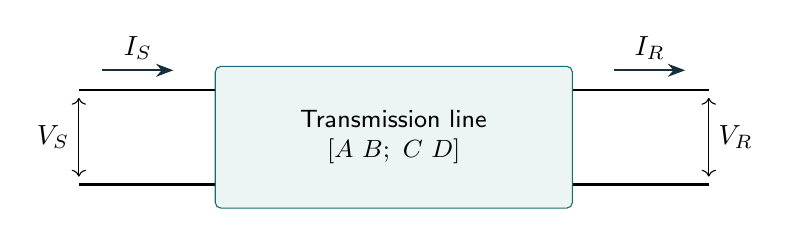
\begin{tikzpicture}
\node[block,text width=4.3cm,minimum height=1.8cm] (line) at (4,0) {Transmission line\\$[A\ B;\ C\ D]$};
\draw[thick] (0,.6)--(line.west |- 0,.6);\draw[thick] (line.east |- 0,.6)--(8,.6);
\draw[thick] (0,-.6)--(line.west |- 0,-.6);\draw[thick] (line.east |- 0,-.6)--(8,-.6);
\draw[arr] (.3,.85)--node[above]{$I_S$}(1.2,.85);
\draw[arr] (6.8,.85)--node[above]{$I_R$}(7.7,.85);
\draw[<->] (0,-.5)--node[left]{$V_S$}(0,.5);
\draw[<->] (8,-.5)--node[right]{$V_R$}(8,.5);
\end{tikzpicture}
\end{center}
\[
 \ans{V_S=AV_R+BI_R},\qquad \ans{I_S=CV_R+DI_R},\qquad
 \begin{bmatrix}V_S\\I_S\end{bmatrix}
 =\begin{bmatrix}A&B\\C&D\end{bmatrix}
 \begin{bmatrix}V_R\\I_R\end{bmatrix}.
\]
All four can be complex. For open circuit $I_R=0$,
\[
 A=\left.\frac{V_S}{V_R}\right|_{I_R=0},\qquad
 C=\left.\frac{I_S}{V_R}\right|_{I_R=0}.
\]
For short circuit $V_R=0$,
\[
 B=\left.\frac{V_S}{I_R}\right|_{V_R=0},\qquad
 D=\left.\frac{I_S}{I_R}\right|_{V_R=0}.
\]
$A,D$ are dimensionless; $B$ has units $\Omega$; $C$ has units S (formerly mho). $C$ is an \textbf{admittance-type transfer constant}, not necessarily a real conductance, despite Part 2 p. 10's wording. It is not the line's capacitance either.
\subsubsection{Open-circuit terminal condition}\slides{Part 2, p. 10}
\begin{center}\includegraphics[width=.94\textwidth,height=68mm,keepaspectratio]{Study_Assets/Module2/p2_010.pdf}\end{center}
\diagramcaption{Set receiving current to zero to identify A and C. Port current directions must match the ABCD definition.}

\subsubsection{Short-circuit terminal condition}\slides{Part 2, p. 11}
\begin{center}\includegraphics[width=.94\textwidth,height=68mm,keepaspectratio]{Study_Assets/Module2/p2_011.pdf}\end{center}
\diagramcaption{Set receiving voltage to zero to identify B and D. This is a parameter-identification condition, not normal loading.}

For a reciprocal network, $\ans{AD-BC=1}$. For a network symmetric between its ports, $\ans{A=D}$. These are different properties. The short, nominal-T, nominal-$\pi$ and uniform distributed line models here have both. Small departures in supplied numerical constants may arise from rounding; a large departure signals inconsistent data or arithmetic.
\subsection{Derive the short-line constants}
With charging omitted, the same current passes through the total series impedance $Z$:
\[
 I_S=I_R,\qquad V_S=V_R+ZI_R.
\]
Read off the coefficients:
\[
 \ans{A=D=1,\quad B=Z,\quad C=0}.
\]
$AD-BC=1$ immediately. At open circuit $I_R=0$, this model predicts no charging current and no Ferranti rise; that is a limitation of the approximation.
\subsubsection{Short-line equivalent}\slides{Part 2, p. 3}
\begin{center}\includegraphics[width=.94\textwidth,height=68mm,keepaspectratio]{Study_Assets/Module2/p2_003.pdf}\end{center}
\diagramcaption{Series Z remains; shunt admittance is neglected. The nominal-T and nominal-pi models are redrawn in Section~\ref{models}.}
\subsection{Derive nominal-T constants with KCL and KVL}
\begin{center}
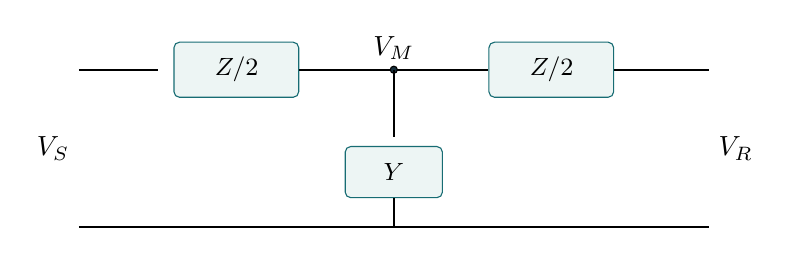
\begin{tikzpicture}
\draw[thick] (0,1)--(1,1);\node[block,text width=1.35cm,minimum height=.7cm] (z1) at (2,1){$Z/2$};
\draw[thick] (z1.east)--(4,1);\node[block,text width=1.35cm,minimum height=.7cm] (z2) at (6,1){$Z/2$};
\draw[thick] (4,1)--(z2.west);\draw[thick] (z2.east)--(8,1);
\draw[fill=ink] (4,1) circle(.045);\node[above] at (4,1){$V_M$};
\draw[thick] (4,1)--(4,.15);\node[block,text width=1cm,minimum height=.65cm] (y) at (4,-.3){$Y$};
\draw[thick] (y.south)--(4,-1);\draw[thick] (0,-1)--(8,-1);
\node[left] at (0,0){$V_S$};\node[right] at (8,0){$V_R$};
\end{tikzpicture}
\end{center}
Work \emph{from receiving end to sending end}:
\[
 V_M=V_R+\frac Z2I_R,
 \qquad I_S=I_R+YV_M
 =YV_R+\left(1+\frac{YZ}{2}\right)I_R.
\]
Then
\[
 \begin{aligned}
 V_S&=V_M+\frac Z2I_S\\
 &=\left(1+\frac{YZ}{2}\right)V_R+
 \left[\frac Z2+\frac Z2\left(1+\frac{YZ}{2}\right)\right]I_R\\
 &=\left(1+\frac{YZ}{2}\right)V_R+Z\left(1+\frac{YZ}{4}\right)I_R.
 \end{aligned}
\]
Therefore
\[
 \ans{A=D=1+\frac{YZ}{2},\quad B=Z\left(1+\frac{YZ}{4}\right),\quad C=Y}.
\]
$Y$ is the \emph{whole-line shunt admittance}; each series arm is $Z/2$. Substituting per-kilometre quantities without first multiplying by line length would produce the wrong constants.
\subsection{Derive nominal-\texorpdfstring{$\pi$}{pi} constants}
\begin{center}
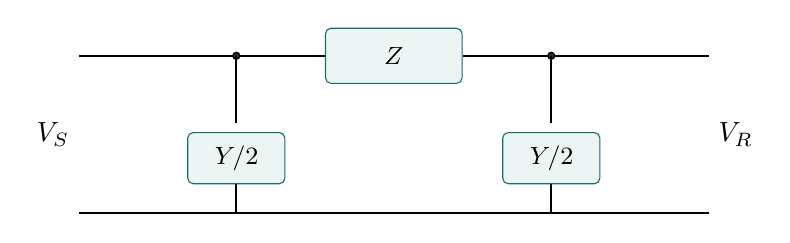
\begin{tikzpicture}
\draw[thick] (0,1)--(2,1);\node[block,text width=1.5cm,minimum height=.7cm] (z) at (4,1){$Z$};
\draw[thick] (2,1)--(z.west);\draw[thick] (z.east)--(8,1);
\foreach \x in {2,6}{
 \draw[fill=ink] (\x,1) circle(.045);\draw[thick] (\x,1)--(\x,.15);
 \node[block,text width=1cm,minimum height=.65cm] (y\x) at (\x,-.3){$Y/2$};
 \draw[thick] (y\x.south)--(\x,-1);}
\draw[thick] (0,-1)--(8,-1);
\node[left] at (0,0){$V_S$};\node[right] at (8,0){$V_R$};
\end{tikzpicture}
\end{center}
The series-branch current is not the load current:
\[
 I_Z=I_R+\frac Y2V_R.
\]
KVL gives
\[
 V_S=V_R+ZI_Z
 =\left(1+\frac{YZ}{2}\right)V_R+ZI_R.
\]
Sending-end KCL gives
\[
 \begin{aligned}
 I_S&=I_Z+\frac Y2V_S\\
 &=Y\left(1+\frac{YZ}{4}\right)V_R+
 \left(1+\frac{YZ}{2}\right)I_R.
 \end{aligned}
\]
Thus
\[
 \ans{A=D=1+\frac{YZ}{2},\quad B=Z,\quad C=Y\left(1+\frac{YZ}{4}\right)}.
\]
A useful memory link is \textbf{T: $C=Y$; $\pi$: $B=Z$}. Both have the same $A,D$, but generally predict different terminal voltage/current because $B,C$ differ.

For either nominal model,
\[
 AD-BC=\left(1+\frac{YZ}{2}\right)^2-YZ\left(1+\frac{YZ}{4}\right)=1.
\]
This verifies the derivation without assuming that T and $\pi$ are exactly the same distributed line.
\subsection{Distributed long line: where hyperbolic constants come from}
The syllabus asks for classification concepts and ABCD derivation/calculation. The class develops the short and nominal models in detail; this subsection supplies the distributed connection for completeness. Let $z'$ and $y'$ be per-length quantities, and measure $x$ from receiving end toward sending end. For an infinitesimal section,
\[
 \frac{dV}{dx}=z'I,\quad \frac{dI}{dx}=y'V,
 \qquad \frac{d^2V}{dx^2}=z'y'V.
\]
Define $\gamma=\sqrt{z'y'}$ and $Z_c=\sqrt{z'/y'}$. Applying $V(0)=V_R$, $I(0)=I_R$ to the general exponential solution yields
\[
 \begin{aligned}
 V(x)&=V_R\cosh(\gamma x)+Z_cI_R\sinh(\gamma x),\\
 I(x)&=\frac{V_R}{Z_c}\sinh(\gamma x)+I_R\cosh(\gamma x).
 \end{aligned}
\]
At $x=\ell$,
\[
 \ans{A=D=\cosh(\gamma\ell)},\quad
 \ans{B=Z_c\sinh(\gamma\ell)},\quad
 \ans{C=\frac1{Z_c}\sinh(\gamma\ell)}.
\]
The identity $\cosh^2u-\sinh^2u=1$ verifies reciprocity. With total $Z=z'\ell$, $Y=y'\ell$, one may compute $u=\sqrt{ZY}$ and $Z_c=\sqrt{Z/Y}$, keeping consistent square-root branches so $Z_cu=Z$. For lossless lines $\gamma=\jj\beta$, $\beta=\omega\sqrt{L'C'}$, so
\[
 A=D=\cos(\beta\ell),\quad B=\jj Z_0\sin(\beta\ell),\quad
 C=\jj\frac{\sin(\beta\ell)}{Z_0},\quad Z_0=\sqrt{L'/C'}.
\]
An exact long-line $\pi$ equivalent uses series $Z_\pi=B$ and each shunt arm $Y_\pi/2=(A-1)/B$. Hence
\[
 Z_\pi=Z_c\sinh u,\qquad Y_\pi/2=\frac1{Z_c}\tanh(u/2).
\]
This is an \emph{equivalent} $\pi$, not a nominal-$\pi$ using uncorrected $Z,Y$. For small $u$, $\cosh u\approx1+ZY/2$ and $\sinh u\approx u$, which explains the nominal approximation.
\subsubsection{Distributed line}\slides{Part 2, p. 6}
\begin{center}\includegraphics[width=.94\textwidth,height=68mm,keepaspectratio]{Study_Assets/Module2/p2_006.pdf}\end{center}
\diagramcaption{A small segment contains series resistance and inductance and shunt conductance and capacitance. The continuous limit produces the long-line equations.}
\subsection{Cascaded and parallel two-port networks}
\slides{Part 2 pp. 17--18}
For network 1 followed by network 2 from sending to receiving end,
\[
 T=T_1T_2,\qquad
 \begin{aligned}
 A&=A_1A_2+B_1C_2,& B&=A_1B_2+B_1D_2,\\
 C&=C_1A_2+D_1C_2,& D&=C_1B_2+D_1D_2.
 \end{aligned}
\]
Order matters in a matrix product. Reciprocity survives cascading because determinants multiply.
\subsubsection{Cascade connection}\slides{Part 2, p. 17}
\begin{center}\includegraphics[width=.94\textwidth,height=68mm,keepaspectratio]{Study_Assets/Module2/p2_017.pdf}\end{center}
\diagramcaption{The output of one network drives the input of the next. Multiply ABCD matrices in their physical order.}

For two reciprocal networks in parallel at both ports, terminal voltages are common and currents add. With nonzero $B_1,B_2$ and $B_1+B_2\ne0$,
\[
 A=\frac{A_1B_2+A_2B_1}{B_1+B_2},\quad
 B=\frac{B_1B_2}{B_1+B_2},\quad
 D=\frac{D_1B_2+D_2B_1}{B_1+B_2},
\]
\[
 C=C_1+C_2-\frac{(A_1-A_2)(D_1-D_2)}{B_1+B_2}.
\]
These follow by writing $I_{Ri}=(V_S-A_iV_R)/B_i$ and summing receiving and sending currents. Alternatively, obtain $C=(AD-1)/B$ for a reciprocal equivalent when $B\ne0$. For two \emph{identical} networks, $A,D$ stay unchanged, $B$ halves and $C$ doubles. Do not multiply transmission matrices for a parallel connection. Separately model mutual coupling if the physical parallel paths are magnetically coupled; these uncoupled two-port-combination formulas do not create that coupling automatically.
\subsubsection{Parallel connection}\slides{Part 2, p. 18}
\begin{center}\includegraphics[width=.94\textwidth,height=68mm,keepaspectratio]{Study_Assets/Module2/p2_018.pdf}\end{center}
\diagramcaption{Both networks share corresponding port voltages. Add admittance matrices, not ABCD matrices.}
\subsection{A numerical workflow you can reuse}
\begin{enumerate}
\item Choose the stated line model and identify per-length versus total parameters.
\item Form $Z$ and $Y$ in compatible units; if given capacitance, first use $Y=\jj\omega C_n$.
\item Compute $A,B,C,D$ in rectangular form, and check units, $A=D$ if appropriate, and $AD-BC\approx1$.
\item Set receiving phase voltage as reference. Determine load current with the correct lag/lead sign.
\item Calculate $V_S,I_S$ as complex sums, then convert magnitudes/angles as required.
\item For regulation, keep $V_S$ fixed and set \emph{load current} $I_R=0$; do not set all line current to zero.
\end{enumerate}

\chapterstart{Voltage regulation, efficiency and class ABCD problems}{performance}
\slides{Part 2 pp. 19--26}
\subsection{Voltage regulation has a specific reference condition}
At fixed sending-end voltage and unchanged line parameters, remove the load. Then $I_R=0$, so $V_{R0}=V_S/A$. Standard transmission-line voltage regulation is
\[
 \ans{\mathrm{VR}=\frac{|V_{R0}|-|V_R|}{|V_R|}\,100\%}
 =\frac{|V_S|/|A|-|V_R|}{|V_R|}\,100\%.
\]
This is the no-load to full-load change \emph{at the receiving end}. The terminal magnitude difference $(|V_S|-|V_R|)/|V_R|$ equals it only when $|A|=1$, as in the short-line model. A leading load can yield negative regulation. Regulation and stability are related to operating voltage but are not the same quantity.
\subsection{Efficiency and sending power factor}
\[
 P_R=3\operatorname{Re}(V_RI_R^*),\quad
 P_S=3\operatorname{Re}(V_SI_S^*),\quad
 \ans{\eta=\frac{P_R}{P_S}100\%}.
\]
Sending power factor is $\cos[\arg V_S-\arg I_S]$. A positive current angle relative to $V_S$ is leading. The receiving power factor need not equal the sending power factor because line charging and inductive absorption alter reactive power.

For a short line with no shunt loss, $P_S=P_R+3|I_R|^2R$. For nominal-T, the two series halves carry different currents, so copper loss is $\tfrac32R(|I_S|^2+|I_R|^2)$. For nominal-$\pi$, series current is $I_Z=I_R+(Y/2)V_R$, and copper loss is $3|I_Z|^2R$ when the shunts are ideal. Do not apply the short-line loss formula to a medium line without checking branch currents.
\subsection{Class Example 6.23: nominal-T constants}
\slides{Part 2 pp. 19--20}
An 80 km, three-phase, 50 Hz line has series impedance $(0.15+\jj0.78)\ \Omega$/km and shunt \emph{admittance} $\jj5\times10^{-6}$ S/km. The source calls this ``shunt capacitance'', but S/km and an imaginary value identify admittance: no extra $\omega$ multiplication is needed.
\[
 Z=80(0.15+\jj0.78)=12+\jj62.4\ \Omega,\quad
 Y=\jj0.0004\ \mathrm S.
\]
\[
 YZ=-0.02496+\jj0.0048,\qquad
 A=D=1+YZ/2=\ans{0.98752+\jj0.0024}.
\]
\[
 \begin{aligned}
 B&=(12+\jj62.4)(0.99376+\jj0.0012)\\
 &=\ans{11.85024+\jj62.025024\ \Omega},\\
 C&=\ans{\jj0.0004\ \mathrm S}.
 \end{aligned}
\]
Check $A^2-BC=1$. The source's printed imaginary part of $B$, approximately 11.91, is an arithmetic error; the direct multiplication gives approximately 62.025. It is also physically sensible that $B$ stays near the original $Z$ for this modest shunt correction.
\Needspace{28\baselineskip}
\subsection{Class Example 6.24: sending end and regulation}
\slides{Part 2 pp. 21--24}
Given $A=D=0.936+\jj0.016$, $B=33.5+\jj138\ \Omega$, $C=(-0.928+\jj901.223)\times10^{-6}$ S. The receiving load is 40 MW at 200 kV, power factor 0.86 lagging; $|V_S|$ remains fixed for the regulation calculation.
\[
 V_R=\frac{200000}{\sqrt3}=115470.054\angle0^\circ\ \mathrm V,
 \quad |I_R|=\frac{40\times10^6}{\sqrt3(200000)(0.86)}=134.2675\ \mathrm A.
\]
\[
 \phi=\cos^{-1}(0.86)=30.68^\circ,\qquad
 I_R=115.4701-\jj68.5159\ \mathrm A.
\]
\[
 \begin{aligned}
 V_S&=AV_R+BI_R=121403.412+\jj15487.105\ \mathrm V,\\
 |V_S|&\approx122387.25\ \mathrm V,\qquad
 \ans{V_{S,LL}=211.981\ \mathrm{kV}},\\
 I_S&=CV_R+DI_R=109.0691+\jj41.7809\ \mathrm A,\\
 \ans{|I_S|}&=\ans{116.798\ \mathrm A}.
 \end{aligned}
\]
$V_S$ angle is approximately $7.27^\circ$; $I_S$ approximately $20.96^\circ$. Current leads sending voltage by $13.69^\circ$, so
\[
 \ans{\mathrm{pf}_S=0.97159\ \text{leading}},\qquad
 P_S=3\operatorname{Re}(V_SI_S^*)=\ans{41.6653\ \mathrm{MW}}.
\]
A useful additional check is $\eta=40/41.6653=\ans{96.003\%}$. For standard regulation,
\[
 |A|=0.9361367,\quad V_{R0,LL}=\frac{211.98094}{0.9361367}=226.4423\ \mathrm{kV},
\]
\[
 \ans{\mathrm{VR}=\frac{226.4423-200}{200}100=13.221\%}.
\]
\begin{Caution}{Why the slide's 5.99\% differs}
Part 2 p. 24 uses $(211.98-200)/200=5.99\%$, the sending-to-receiving terminal magnitude difference. With $|A|\ne1$, that is not the standard fixed-sending-voltage no-load regulation. Both numbers can be reported if clearly labelled, but 13.22\% answers the standard definition. The supplied rounded constants satisfy $AD-BC\approx1.000240-\jj0.000111$, so retain the given data rather than claiming perfect exact reciprocity.
\end{Caution}
\chapterstart{Ferranti effect and corona}{phenomena}
\slides{Part 2 pp. 32--50}
\subsection{Ferranti effect: why open circuit can raise voltage}
\textbf{Ferranti effect} is receiving-end voltage exceeding sending-end voltage under no load or light load, due to the combination of line capacitance and inductance. It is appreciable in medium/long overhead lines and can matter in cables with large capacitance. A short model omits the charging path and cannot reproduce it.

Let $V_R$ be the reference. Capacitive current is $I_c=\jj\omega CV_R$. Its series inductive drop is
\[
 (\jj\omega L)I_c=(\jj\omega L)(\jj\omega CV_R)
 =-\omega^2LCV_R.
\]
The drop points opposite to $V_R$, so $V_S$ can have smaller magnitude. Resistance adds a quadrature term; it is not the main cause of the rise. No energy is created: voltage changes through reactive field exchange, while the ideal no-load line transfers no real power to a load.
\subsubsection{Ferranti physical picture}\slides{Part 2, p. 33}
\begin{center}\includegraphics[width=.94\textwidth,height=68mm,keepaspectratio]{Study_Assets/Module2/p2_033.pdf}\end{center}
\diagramcaption{At no load, distributed charging current still flows and the receiving voltage can exceed sending voltage.}
\begin{center}
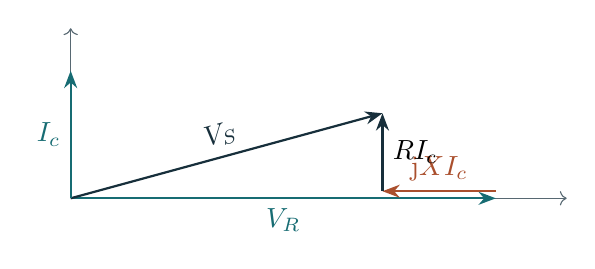
\begin{tikzpicture}[scale=.9]
\draw[->,muted] (0,0)--(7,0);\draw[->,muted] (0,0)--(0,2.4);
\draw[arr,teal] (0,0)--node[below]{$V_R$}(6,0);
\draw[arr,rust] (6,.1)--node[above]{$\jj X I_c$}(4.4,.1);
\draw[arr] (4.4,.1)--node[right]{$RI_c$}(4.4,1.2);
\draw[arr,ink] (0,0)--node[above,sloped]{$V_S$}(4.4,1.2);
\draw[arr,teal] (0,0)--node[left]{$I_c$}(0,1.8);
\end{tikzpicture}
\end{center}
\diagramcaption{A conceptual charging-current phasor construction, not to scale. For a distributed line, the effective series current varies along the line; the nominal model determines how it is represented.}
\subsubsection{Ferranti phasors}\slides{Part 2, p. 36}
\begin{center}\includegraphics[width=.94\textwidth,height=68mm,keepaspectratio]{Study_Assets/Module2/p2_036.pdf}\end{center}
\diagramcaption{With receiving voltage as reference, charging current leads by 90 degrees. The reactive series voltage points opposite to receiving voltage; resistive voltage follows charging current.}
\subsection{Obtain a consistent rise formula}
For no load in nominal-T or nominal-$\pi$,
\[
 V_S=AV_R,\qquad A=1+ZY/2.
\]
Neglect $R,G$ and use \emph{total} $L,C$:
\[
 A=1-\omega^2LC/2,\qquad
 \frac{V_R-V_S}{V_R}\approx\frac{\omega^2LC}{2}
 =\frac{\omega^2L'C'\ell^2}{2}.
\]
For a lossless distributed line, the exact expression is
\[
 V_S=V_R\cos(\beta\ell),\qquad
 \frac{V_R-V_S}{V_R}=1-\cos(\beta\ell),\quad
 \beta=\omega\sqrt{L'C'}.
\]
Using $\cos x\approx1-x^2/2$ gives the same approximate result. The \textbf{factor $1/2$} reflects distributed charging; the all-capacitance-at-the-receiving-end lumped model gives a different approximation. Do not mix that simplified sketch with the more accurate formula as Part 2 p. 37 does. Pages 38--39 provide the consistent half-factor derivation.

Assuming overhead wave speed $v\approx3\times10^8$ m/s, $L'C'\approx1/v^2$:
\[
 \frac{V_R-V_S}{V_R}\approx\frac{\omega^2\ell_{\rm m}^2\,10^{-16}}{18}
 =\frac{\omega^2\ell_{\rm km}^2\,10^{-10}}{18}.
\]
If expressing rise as a percentage of $V_S$, rather than $V_R$, use $(V_R/V_S-1)100$; the two differ slightly. State the reference when accuracy matters.
\subsubsection{Ferranti waveforms}\slides{Part 2, p. 40}
\begin{center}\includegraphics[width=.94\textwidth,height=68mm,keepaspectratio]{Study_Assets/Module2/p2_040.pdf}\end{center}
\diagramcaption{The voltage rise is explained by phasor addition. Use the half-length charging-current approximation in the main derivation; a lumped total current gives the wrong factor.}
\subsection{Class Example 6.22: 200 km at 50 Hz}
\slides{Part 2 pp. 42--43}
With the slide's overhead wave-speed assumption,
\[
 \frac{\Delta V}{V_R}100
 \approx\frac{(2\pi50)^2(200)^2\,10^{-10}}{18}100
 =\ans{2.19325\%}.
\]
No nominal voltage is needed because it cancels. The exact lossless model gives $1-\cos(2\pi50\times200000/(3\times10^8))=2.18524\%$ of $V_R$; relative to $V_S$ the rise is about 2.23406\%. In the class's approximate calculation, quote \textbf{2.19\%} and name the assumptions.
\subsection{Consequences and mitigation}
Light-load overvoltage stresses transformers, switchgear and insulators; operating voltage may exceed desired limits. Shunt reactors absorb the capacitive reactive output and control the rise. Suitable loading, switching and coordinated voltage control also help. A stated percentage rise for a 300 km line is an illustrative estimate depending on its parameters, frequency and loading, not an automatic value determined by distance alone.
\subsection{Corona: the qualitative answer required by the syllabus}
\textbf{Corona} is local air ionisation around a high-voltage conductor or fitting when the local electric field exceeds the onset threshold. It may produce a violet/blue glow, hissing/crackling, ozone, radio interference and power loss. The photos in Part 2 pp. 44--45 show local discharge, not useful energy generation.

Onset depends on \textbf{electric field}, not a single universal line-voltage cutoff. Higher voltage, a small radius, surface roughness/sharp fittings and unfavourable atmospheric conditions can increase discharge. Air density, altitude, rain/wet surfaces and contamination matter; weather effects should not be reduced to one humidity rule. Increasing conductor diameter, using bundles and smoothing fittings reduce local field stress. Increasing phase spacing can help within the corresponding geometry.

\textbf{Disruptive critical voltage} denotes corona onset; \textbf{visual critical voltage} denotes a visible discharge under the stated conditions. Onset need not be visibly obvious. Corona is a local partial discharge; \textbf{flashover} is a complete discharge path across an air/surface insulation gap. They are not interchangeable.

\textbf{Disadvantages:} wasted real power, audible noise, electromagnetic interference and chemical/insulation deterioration. Discharge pulses contain non-sinusoidal components and can disturb communication channels. Long-term effects depend on the insulation and discharge location.

\textbf{The class's possible beneficial effect:} corona can dissipate some energy from a travelling surge and modify local effective electric-field distribution. Treat this as a secondary physical effect. It is not a dependable protection device, and it does not guarantee reduced flashover or replace surge arresters and insulation coordination. Avoid the blanket claim that corona improves reliability. Numerical Peek-law loss or critical-voltage derivations are outside the syllabus's \emph{qualitative} corona scope.
\subsubsection{Corona on fittings}\slides{Part 2, p. 44}
\begin{center}\includegraphics[width=.94\textwidth,height=68mm,keepaspectratio]{Study_Assets/Module2/p2_044.pdf}\end{center}
\diagramcaption{The class photograph illustrates visible discharge at regions of high surface electric field.}

\subsubsection{Corona along a line}\slides{Part 2, p. 45}
\begin{center}\includegraphics[width=.94\textwidth,height=68mm,keepaspectratio]{Study_Assets/Module2/p2_045.pdf}\end{center}
\diagramcaption{Violet glow is a recognition aid; inception depends on geometry, surface condition and atmosphere, not a universal voltage threshold.}
\checkq{Are Ferranti effect and corona both losses caused by high voltage?}{No. Ferranti effect is a reactive voltage-rise phenomenon involving line $L,C$ under light load. Corona is local ionisation that can cause real loss, noise and interference when electric-field stress is excessive.}

\chapterstart{Surge impedance and natural loading}{sil}
\slides{Part 2 pp. 51--58}
\subsection{Derive SIL from reactive balance}
For a nearly uniform lossless line, per-length inductive absorption magnitude is $Q_L'=\omega L'|I|^2$, while capacitive supply is $Q_C'=\omega C'|V_{\rm ph}|^2$. Equating them gives
\[
 L'|I|^2=C'|V_{\rm ph}|^2,\qquad
 \ans{\frac{|V_{\rm ph}|}{|I|}=\sqrt{\frac{L'}{C'}}=Z_0}.
\]
With a real characteristic-impedance termination, $I=V_{\rm ph}/Z_0$ in phase, so
\[
 P_{\rm SIL,ph}=\frac{V_{\rm ph}^2}{Z_0},\qquad
 \ans{P_{\rm SIL,3\phi}=3\frac{V_{\rm ph}^2}{Z_0}=\frac{V_{LL}^2}{Z_0}}.
\]
With $V_{LL}$ in kV and $Z_0$ in ohms, the answer is directly in MW. $L'$ and $C'$ must refer to the same phase model and same per-length unit. Using total $L,C$ gives the same ratio if both scale with the same length.

For a lossy line the general characteristic impedance is $Z_c=\sqrt{z'/y'}$, usually complex. The real $\sqrt{L'/C'}$ is the lossless surge-impedance approximation. A real $Z_0$ is not a literal line resistance dissipating $I^2Z_0$: it is a voltage/current ratio associated with travelling fields.

\begin{Caution}{Which voltage appears across the line inductor?}
The class infographics in Part 2 pp. 52--53 write an inductive expression involving $V^2/(\omega L)$. If $V$ means phase-to-neutral line voltage, that does not describe the series inductor's absorption. Its correct expression is $I^2\omega L$; $V_X^2/(\omega L)$ would use the voltage \emph{across the inductor}. Starting with $Q_L=I^2\omega L$ and $Q_C=V^2\omega C$ gives the correct $Z_0$ above.
\end{Caution}
\subsection{Below, at and above SIL}
\begin{center}\small
\begin{tabularx}{\textwidth}{L{2.9cm}YY}
\toprule\textbf{Loading} & \textbf{Net line reactive tendency} & \textbf{Voltage tendency}\\\midrule
Below SIL & Capacitive supply exceeds inductive absorption & Voltage rise/light-load overvoltage tendency.\\
At SIL & Equal generation and absorption in the ideal lossless, matched case & Flat voltage magnitude; phase angle still changes with distance.\\
Above SIL & Inductive absorption exceeds capacitive supply & Voltage-drop/reactive-support tendency.\\\bottomrule
\end{tabularx}\end{center}
These are natural-loading comparisons under the ideal assumptions. Actual terminal voltage depends on power factor, compensation, regulated buses and resistance. At ideal SIL, $|V_S|=|V_R|$; they are not identical phasors because a propagation angle exists. No line-generated net var does not mean every connected load has zero reactive demand.
\Needspace{23\baselineskip}
\subsection{Class SIL example: 220 kV line}
\slides{Part 2 pp. 57--58}
Given $L'=1.2$ mH/km and $C'=0.01\ \mu$F/km:
\[
 Z_0=\sqrt{\frac{1.2\times10^{-3}}{0.01\times10^{-6}}}
 =\ans{346.410\ \Omega}.
\]
\[
 P_{\rm SIL,3\phi}=\frac{220^2}{346.410}=\ans{139.719\ \mathrm{MW}}.
\]
Per-phase SIL is $46.573$ MW. At 80 MW ($<139.719$), the uncompensated line tends to supply vars and raise voltage; at 250 MW ($>139.719$), it tends to absorb vars and lower voltage. The source's approximately 139.5 MW follows rounding $220/\sqrt3$ to 127 kV.
\subsection{SIL is not a maximum power rating}
Thermal ampacity, steady-state/transient stability, voltage constraints, insulation and operating contingencies determine allowable power transfer. A line may operate above or below SIL. Bundles generally increase $C'$ and reduce $L'$, lowering $Z_0$ and increasing SIL for fixed voltage. The class's typical overhead/cable impedance values are illustrative; values vary with conductor geometry and dielectric construction. Do not use a memorised 400 or 600 $\Omega$ when a problem gives $L',C'$.

\chapterstart{Insulators and voltage distribution}{insulators}
\slides{Part 2 pp. 59--78}
\subsection{Functions, materials and types}
Bare overhead conductors need both mechanical support and electrical separation from grounded tower steelwork. Insulators sustain conductor weight/tension, preserve air clearance and restrict leakage/discharge. Selection includes working voltage, impulse withstand, mechanical load, pollution, wet-weather behaviour and maintenance.

Porcelain, toughened glass and composite/polymer constructions serve different environments. Sheds extend \textbf{creepage distance}, the path along the surface; \textbf{clearance} is distance through air. A polluted wet surface can conduct despite a sound bulk material. Flashover is an external/surface discharge; puncture passes through the insulator body and may cause permanent damage.
\begin{center}\small
\begin{tabularx}{\textwidth}{L{2.8cm}Y}
\toprule\textbf{Type} & \textbf{Purpose and recognition}\\\midrule
Pin & Mounted on a support pin with a conductor groove; common in lower-voltage overhead construction.\\
Suspension & Hanging string or long-rod arrangement; supports conductor with several units where appropriate for higher voltage.\\
Strain & Arranged to sustain tensile forces at dead ends/large direction changes; disc strings may be oriented approximately horizontally.\\
Shackle & Compact spool-type support used in low-voltage distribution and at bends/ends.\\
Post (slide photograph) & Rigid support for conductors/buswork in suitable line or station applications.\\
Stay (slide photograph) & Isolates an accessible part of a guy/stay wire from hazardous energisation.\\\bottomrule
\end{tabularx}\end{center}
The class photographs in pp. 62--63 show material and mechanical arrangements. An arcing horn provides a preferred external arc path under specified conditions; a grading/corona ring controls electric-field distribution. These are related line accessories with different functions.
\subsubsection{Insulator type gallery}\slides{Part 2, p. 62}
\begin{center}\includegraphics[width=.94\textwidth,height=68mm,keepaspectratio]{Study_Assets/Module2/p2_062.pdf}\end{center}
\diagramcaption{Recognize glass/disc, post, pin, shackle, strain, stay and suspension forms. The four syllabus-focused forms are explained in the main text.}

\subsubsection{Mechanical string and electrical equivalent}\slides{Part 2, p. 63}
\begin{center}\includegraphics[width=.94\textwidth,height=68mm,keepaspectratio]{Study_Assets/Module2/p2_063.pdf}\end{center}
\diagramcaption{Match metal links to shunt capacitances, and each insulating disc to series capacitance. Arcing horns provide a controlled external flashover path.}
\subsection{The string's capacitive equivalent circuit}
Number discs from \textbf{tower end} to \textbf{line end}. Each identical disc has self-capacitance $C_d$. Every intermediate metal fitting has shunt capacitance $kC_d$ to the grounded tower. In the elementary model neglect surface leakage conductance and capacitance to the live conductor; later a guard ring deliberately changes that field coupling.
\begin{center}
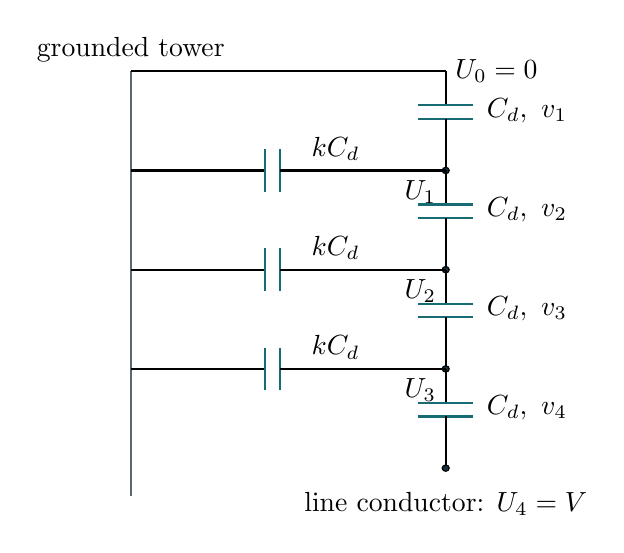
\begin{tikzpicture}[x=1cm,y=.9cm]
\draw[thick,muted] (0,0)--(0,-6);\node[above] at (0,0){grounded tower};
\draw[thick] (0,0)--(4,0);\node[right] at (4,0){$U_0=0$};
\foreach \j in {1,2,3,4}{
 \pgfmathsetmacro{\ytop}{-1.4*(\j-1)}\pgfmathsetmacro{\ybot}{-1.4*\j}
 \draw[thick] (4,\ytop)--(4,\ytop-.48);
 \draw[thick,teal] (3.65,\ytop-.48)--(4.35,\ytop-.48);
 \draw[thick,teal] (3.65,\ytop-.67)--(4.35,\ytop-.67);
 \draw[thick] (4,\ytop-.67)--(4,\ybot);
 \node[right] at (4.4,\ytop-.55){$C_d,\ v_\j$};
 \draw[fill=ink] (4,\ybot) circle(.045);
}
\foreach \j in {1,2,3}{
 \pgfmathsetmacro{\y}{-1.4*\j}
 \draw[thick] (0,\y)--(1.7,\y);\draw[teal,thick] (1.7,\y-.3)--(1.7,\y+.3);
 \draw[teal,thick] (1.9,\y-.3)--(1.9,\y+.3);\draw[thick] (1.9,\y)--(4,\y);
 \node[above] at (2.6,\y){$kC_d$};\node[below left] at (4,\y){$U_\j$};
}
\node[below] at (4,-5.8){line conductor: $U_4=V$};
\end{tikzpicture}
\end{center}
Let $v_j=U_j-U_{j-1}$, so $U_j=v_1+\cdots+v_j$. Disc current from below is $\jj\omega C_d v_{j+1}$; it splits into upper-disc current $\jj\omega C_dv_j$ and tower current $\jj\omega kC_dU_j$. Cancelling $\jj\omega C_d$ gives the fundamental recurrence:
\[
 \ans{v_{j+1}=v_j+k\sum_{i=1}^{j}v_i}.
\]
This derivation prevents the common mistake of using only $kv_j$ as the shunt contribution. The fitting's voltage to ground is \emph{cumulative voltage} $U_j$, not merely the voltage of the adjacent disc.
\subsection{Derive three- and four-disc distribution}
Taking the top disc voltage as $v_1$,
\[
 \begin{aligned}
 v_2&=v_1+kv_1=(1+k)v_1,\\
 v_3&=v_2+k(v_1+v_2)=(1+3k+k^2)v_1,\\
 v_4&=v_3+k(v_1+v_2+v_3)=(1+6k+5k^2+k^3)v_1.
 \end{aligned}
\]
For three discs,
\[
 V=(3+4k+k^2)v_1,
 \quad \ans{\eta_3=\frac{3+4k+k^2}{3(1+3k+k^2)}100\%}.
\]
For four discs,
\[
 V=(4+10k+6k^2+k^3)v_1,
 \quad \ans{\eta_4=\frac{4+10k+6k^2+k^3}{4(1+6k+5k^2+k^3)}100\%}.
\]
The general definition is
\[
 \ans{\eta=\frac{\text{total string voltage}}{n\,\max(v_j)}100\%}.
\]
In the ungraded tower-shunt model with $k>0$, $v_1<v_2<\cdots<v_n$, so the bottom disc is most stressed. As $k\to0$, all voltages become equal and $\eta\to100\%$. String efficiency describes voltage utilisation, \emph{not energy conversion}. Adding discs under fixed $k$ in this simple model tends to reduce efficiency; actual grading and geometry can change that tendency. The slide's 80--90\% typical values are not a guarantee for every ungraded string.

The coefficients $1,3,6$ of $k$ are triangular numbers for the first four ratios. Keep the full polynomials for ungraded strings; capacitance grading below follows a different, purely linear-in-$k$ formula.
\subsubsection{Four-disc string and earth capacitance}\slides{Part 2, p. 65}
\begin{center}\includegraphics[width=.94\textwidth,height=68mm,keepaspectratio]{Study_Assets/Module2/p2_065.pdf}\end{center}
\diagramcaption{Equal series discs do not give equal voltages when their junctions have earth capacitance. Disc voltage rises towards the conductor.}
\subsection{Improving string efficiency}
\textbf{Longer cross arms} move the string away from the tower and reduce shunt capacitance. \textbf{Higher disc self-capacitance} lowers $k=C_{\rm sh}/C_d$ if shunt geometry is otherwise unchanged; a larger disc does not automatically preserve every other parameter. \textbf{Capacitance grading} deliberately changes disc capacitance along the string. \textbf{Guard/grading rings} connected to the line conductor reshape the field and alter fittings' capacitance to the live line, reducing concentrated stress. They are not simply an added shunt to earth; increasing tower capacitance would worsen this elementary distribution.
\subsection{Derive ideal capacitance grading for any number of discs}
Require each disc to have the same voltage $v=V/n$. Let top disc capacitance be $C_1=C_0$, and every intermediate fitting have the same tower capacitance $C_g=kC_0$. The fitting after $j$ discs has $U_j=jv$.

KCL at that fitting gives
\[
 \jj\omega C_{j+1}v=\jj\omega C_jv+\jj\omega C_g(jv),
 \quad C_{j+1}=C_j+jC_g.
\]
Summing the increments,
\[
 \ans{C_j=C_0+\frac{j(j-1)}2C_g
 =C_0\left[1+\frac{j(j-1)}2k\right]}.
\]
For four discs, the ratio is $1:(1+k):(1+3k):(1+6k)$. Capacitance increases toward the line end because the lower disc must carry upper-disc current plus accumulated tower charging currents, while keeping the same voltage. The ideal model gives $100\%$ efficiency. Different disc sizes/capacitances complicate manufacture, replacement and maintenance.

This formula assumes constant \emph{absolute} $C_g$. If a problem instead makes the shunt at each node a fixed fraction of that node's varying disc capacitance, rederive KCL; the formula changes. ``Self'' and ``mutual'' are used inconsistently in old insulator texts: identify the actual branch capacitance in the diagram rather than trusting the name.
\subsubsection{Capacitance grading circuit}\slides{Part 2, p. 71}
\begin{center}\includegraphics[width=.94\textwidth,height=68mm,keepaspectratio]{Study_Assets/Module2/p2_071.pdf}\end{center}
\diagramcaption{Different disc capacitances give equal intended disc voltages. The caption C1 on the shunt branches refers to the top-unit reference capacitance.}
\subsection{Class Example 3.4: four-disc voltage percentages}
\slides{Part 2 pp. 73--74}
Disc self-capacitance is four times pin-to-earth capacitance, so $k=1/4=0.25$. Relative voltages from tower to conductor are
\[
 v_1:v_2:v_3:v_4=1:1.25:1.8125:2.828125.
\]
Their sum is $6.890625$. Divide each by the sum:
\begin{center}\small
\begin{tabular}{ccccc}
\toprule Disc from tower & 1 & 2 & 3 & 4\\\midrule
Fraction of string voltage & 0.145125 & 0.181406 & 0.263039 & 0.410431\\
Percentage & 14.5125\% & 18.1406\% & 26.3039\% & 41.0431\%\\\bottomrule
\end{tabular}\end{center}
\[
 \eta=\frac{6.890625}{4(2.828125)}100=\ans{60.9116\%}.
\]
Percentages sum to 100\%. The source's 60.92\% is essentially a rounding difference. No system voltage is required because only fractional distribution and efficiency are asked.
\subsection{Class Example 3.9: a six-unit graded string}
\slides{Part 2 pp. 75--76}
Every pin-to-earth capacitance equals $C_g=C$; the top unit's \emph{disc} capacitance is $C_0=10C$. Equal-voltage grading requires
\[
 C_j=10C+\frac{j(j-1)}2C.
\]
Hence, from tower to line,
\[
 \ans{C_1,C_2,C_3,C_4,C_5,C_6=10C,11C,13C,16C,20C,25C}.
\]
At node 5, for example, $C_6v=C_5v+C(5v)$, so $C_6=20C+5C=25C$. The grading ratio is $1:1.1:1.3:1.6:2:2.5$ relative to the top disc. Each disc carries different current but the same voltage; ideal efficiency is 100\%.

\chapterstart{Additional worked examples that connect the ideas}{extraexamples}
These examples are original practice problems, separate from the numbered examples reproduced and recalculated from class. Try each first, then compare the sequence of decisions with the solution.
\subsection{Temperature correction and parallel conductors}
An aluminium conductor has area $300\ \mathrm{mm^2}$, $\rho_{20}=2.83\times10^{-8}\ \Omega\mathrm m$ and $\alpha_{20}=0.00403/{}^\circ\mathrm C$. Find the ideal DC resistance of 1 km at $75{}^\circ\mathrm C$, then that of two parallel circuits, each containing a twin bundle per phase, assuming equal sharing.
\[
 R_{20}=\frac{2.83\times10^{-8}(1000)}{300\times10^{-6}}=0.094333\ \Omega,\qquad
 R_{75}=0.094333[1+0.00403(75-20)]=\ans{0.115242\ \Omega}.
\]
Four equal resistive paths carry the total phase current, so $R_{\mathrm{eq},75}=R_{75}/4=\ans{0.0288106\ \Omega/km}$. Real AC resistance also depends on strand geometry, skin/proximity effects, and any magnetic core; this ideal calculation isolates temperature and parallel sharing. For a line of $\ell$ km, use $3I_{\rm total}^2R_{\rm eq}\ell$ for three-phase loss.

\subsection{One double-circuit geometry, two different self distances}
Consider the reverse-phase vertical arrangement derived in Section~\ref{doubleL}: vertical gap $d_1=3$ m, horizontal gap $d_2=6$ m and solid-conductor radius $r=0.01$ m. Both circuits are in parallel and carry equal shares of each phase current. Find equivalent $L$ and $C$ per phase per km, neglecting earth.
\[
 s=\sqrt{4d_1^2+d_2^2}=\sqrt{72}=8.48528\ \mathrm m,\quad
 D_{AB}=D_{BC}=[d_1^2(d_1^2+d_2^2)]^{1/4}=4.48605\ \mathrm m,
\]
\[
 D_{CA}=\sqrt{2d_1d_2}=6\ \mathrm m,\qquad D_m=(D_{AB}D_{BC}D_{CA})^{1/3}=4.94265\ \mathrm m.
\]
For inductance use $r'=0.778801r$, hence
\[
 D_{sL}=[(r's)^2(r'd_2)]^{1/6}=0.242639\ \mathrm m,\quad
 L=0.2\ln\frac{4.94265}{0.242639}=\ans{0.602816\ \mathrm{mH/km}}.
\]
For capacitance replace $r'$ by the physical $r$:
\[
 D_{sC}=[(rs)^2(rd_2)]^{1/6}=0.274946\ \mathrm m,\quad
 C=\frac{55.632}{\ln(4.94265/0.274946)}=\ans{19.2559\ \mathrm{nF/km}}.
\]
These already refer to total phase current and combined phase charge. Dividing $L$ by two or doubling $C$ once again would count the parallel grouping twice. The two self distances differ because internal magnetic flux affects $L$, whereas electrostatic potential is evaluated at the actual surface.

\subsection{What a grading ring balances in the ideal three-disc model}
Suppose a ring introduces capacitance $C_{\ell j}$ from intermediate node $j$ to the line conductor. For equal disc voltage $v$, node $j$ is at $jv$ from the tower and $(n-j)v$ from the line. The ring branch balances tower charging when
\[
 kC_d(jv)=C_{\ell j}[(n-j)v]\quad\Rightarrow\quad
 C_{\ell j}=kC_d\frac{j}{n-j}.
\]
For three discs, ideal balancing values at nodes 1 and 2 are $kC_d/2$ and $2kC_d$. This deliberately simplified capacitance model explains the \emph{direction} of the ring's effect. Practical ring shape is designed from the electric-field distribution; an actual ring does not supply arbitrarily independent branch capacitances.


\Needspace{27\baselineskip}
\subsection{A complete short-line calculation}
A short line with $Z=4+\jj10\ \Omega$/phase supplies $10$ MW at $33$ kV line-to-line, $0.8$ lagging. Find sending voltage, efficiency and regulation. Take receiving phase voltage as reference.
\[
 V_R=\frac{33000}{\sqrt3}=19052.56\ \mathrm V,\qquad
 I_R=\frac{10\times10^6}{\sqrt3(33000)(0.8)}(0.8-\jj0.6)
 =174.9546-\jj131.2160\ \mathrm A.
\]
With $A=D=1$, $B=Z$, $C=0$:
\[
 V_S=V_R+ZI_R=21064.54+\jj1224.68\ \mathrm V,
 \quad \ans{V_{S,LL}=36.5465\ \mathrm{kV}},\quad \angle V_S=3.3274^\circ.
\]
\[
 P_{\rm loss}=3|I_R|^2(4)=0.573921\ \mathrm{MW},\quad
 P_S=10.573921\ \mathrm{MW},\quad \ans{\eta=94.5723\%}.
\]
At fixed $V_S$, no-load $V_{R0}=V_S/A=V_S$. Thus
\[
 \ans{\mathrm{VR}=\frac{36.5465-33}{33}100=10.7468\%}.
\]
Here the terminal-voltage difference happens to equal true regulation because $A=1$. That shortcut did not work in Class Example 6.24, where $|A|\ne1$.

\subsection{Exact long-line constants and no-load voltage}
A lossless 300 km line has $L'=1$ mH/km, $C'=0.01\ \mu$F/km and $f=50$ Hz. These are \emph{per-km} values; do not multiply by 1000 unless also converting length to metres.
\[
 Z_0=\sqrt{\frac{0.001}{10^{-8}}}=316.2278\ \Omega,\quad
 \theta=\beta\ell=2\pi50\sqrt{0.001(10^{-8})}(300)=0.298038\ \mathrm{rad}.
\]
\[
 \ans{A=D=0.955915},\qquad
 \ans{B=\jj92.8587\ \Omega},\qquad
 \ans{C=\jj0.000928587\ \mathrm S}.
\]
Check $AD-BC=\cos^2\theta+\sin^2\theta=1$. If $V_{S,LL}=220$ kV at no load, $V_{R,LL}=220/A\approx230.146$ kV. The rise relative to sending voltage is $\ans{4.61186\%}$. SIL is $220^2/316.2278=153.054$ MW. SIL refers to natural loading at a stated voltage; the preceding result is the very different \emph{unloaded} operating condition.

\subsection{Inferring insulator earth capacitance from measurements}
For three equal discs, measured voltages from the tower are $v_1=8$ kV and $v_2=11$ kV. Assume only equal disc capacitance $C_d$ and equal intermediate-node earth capacitance $kC_d$.
\[
 k=\frac{v_2}{v_1}-1=0.375,\qquad
 v_3=(1+3k+k^2)v_1=18.125\ \mathrm{kV}.
\]
\[
 V_{\rm phase}=8+11+18.125=37.125\ \mathrm{kV},\quad
 \ans{V_{LL}=\sqrt3(37.125)=64.3024\ \mathrm{kV}},
\]
\[
 \ans{\eta=\frac{37.125}{3(18.125)}100=68.2759\%}.
\]
If the line-end disc is rated for at most 20 kV under this ideal voltage-sharing model, maximum string phase voltage is $20(37.125/18.125)=40.9655$ kV. Real insulation selection also considers pollution, impulse withstand and safety margins; this is a voltage-distribution calculation, not a hardware specification.

\chapterstart{Revision sheets and mistakes to avoid}{revision}
\subsection{Line-parameter formula sheet}
Use SI quantities inside logarithms and form a dimensionless ratio. Natural logarithms are used throughout. The constants below assume air, nonmagnetic solid conductors where applicable, and the stated transposition/grouping model.
\begin{center}\small
\begin{tabularx}{\textwidth}{L{.37\textwidth}Y}
\toprule Quantity & Formula and interpretation\\\midrule
Resistance & $R=\rho\ell/A$; $R_T=R_{T_0}[1+\alpha_{T_0}(T-T_0)]$.\\
Solid-wire magnetic self radius & $r'=e^{-1/4}r=0.778801r$. Internal $L=\mu_0/(8\pi)$ H/m.\\
One conductor, reference return & $L=2\times10^{-7}\ln(D/r')$ H/m.\\
Two-wire loop & $L_{\rm loop}=4\times10^{-7}\ln(D/r')$ H/m for equal wires.\\
Transposed three-phase & $D_m=(D_{ab}D_{bc}D_{ca})^{1/3}$; $L=0.2\ln(D_m/D_s)$ mH/km.\\
Group self/mutual distances & $D_s=(\prod_{i=1}^n\prod_{j=1}^nD_{ij})^{1/n^2}$, $D_{ii}=r'$ for $L$, $r$ for $C$; $D_{XY}=(\prod_{i=1}^n\prod_{j=1}^mD_{ij})^{1/(nm)}$.\\
Double-circuit group model & $D_s=(D_{sA}D_{sB}D_{sC})^{1/3}$, $D_m=(D_{AB}D_{BC}D_{CA})^{1/3}$. Equal sharing and transposition assumptions required.\\
Bundle self radius & Twin: $\sqrt{r_s d}$; equilateral triple: $(r_s d^2)^{1/3}$; square quadruple: $(\sqrt2r_s d^3)^{1/4}$. Use $r_s=r'$ for $L$, $r_s=r$ for $C$.\\
Two-wire capacitance & $C_{LL}=\pi\epsilon_0/\ln(D/r)$; each wire to neutral $C_n=2C_{LL}$.\\
Three-phase phase-neutral $C$ & $C=2\pi\epsilon_0/\ln(D_m/D_{sC})$ F/m $=55.632/\ln(D_m/D_{sC})$ nF/km.\\
Charging quantities & $X_C=1/(\omega C)$; $I_c=\omega CV_{\rm phase}$; $Q_c=3\omega C V_{\rm phase}^2=\omega CV_{LL}^2$.\\\bottomrule
\end{tabularx}\end{center}

\subsection{ABCD, performance and natural loading}
\[
 \begin{bmatrix}V_S\\I_S\end{bmatrix}=
 \begin{bmatrix}A&B\\C&D\end{bmatrix}\begin{bmatrix}V_R\\I_R\end{bmatrix},\quad
 AD-BC=1\ \text{(reciprocal)},\quad A=D\ \text{(symmetric)}.
\]
$A,D$ are dimensionless; $B$ is in ohms; $C$ is in siemens. In these equations $I_R$ flows \emph{out} of the line into its load. $Z$ and $Y$ below are total per-phase line values, whereas $z$ and $y$ in the exact model are per unit length.
\begin{center}\small
\begin{tabular}{lcccc}
\toprule Model & $A$ & $B$ & $C$ & $D$\\\midrule
Short & $1$ & $Z$ & $0$ & $1$\\
Nominal T & $1+YZ/2$ & $Z(1+YZ/4)$ & $Y$ & $1+YZ/2$\\
Nominal $\pi$ & $1+YZ/2$ & $Z$ & $Y(1+YZ/4)$ & $1+YZ/2$\\
Exact long & $\cosh\gamma\ell$ & $Z_0\sinh\gamma\ell$ & $\sinh\gamma\ell/Z_0$ & $\cosh\gamma\ell$\\\bottomrule
\end{tabular}\end{center}
\[
 \gamma=\sqrt{zy},\quad Z_0=\sqrt{z/y};\qquad
 \text{lossless:}\quad Z_0=\sqrt{L'/C'},\quad\gamma=\jj\omega\sqrt{L'C'}=\jj\beta.
\]
\[
 \mathrm{VR}=\frac{|V_S/A|-|V_R|}{|V_R|}100,\quad
 \eta=\frac{P_R}{P_S}100,\quad P_S=3\Re(V_S I_S^*).
\]
\[
 \mathrm{SIL}=V_{LL}^2/Z_0;\qquad
 \frac{V_R-V_S}{V_R}\approx\frac{\omega^2L'C'\ell^2}{2}
 \quad\text{(lossless, unloaded, small electrical length)}.
\]
Cascade matrices in the physical sending-to-receiving order. For parallel branches, add admittance matrices, then convert back; do not add ABCD entries directly.

\subsection{Insulator formula sheet}
Number discs from the earthed tower downward. $k=C_g/C_d$, and $v_j$ is the voltage \emph{across disc} $j$, not the voltage of node $j$ to earth.
\[
 v_2=(1+k)v_1,\quad v_3=(1+3k+k^2)v_1,\quad
 v_4=(1+6k+5k^2+k^3)v_1.
\]
\[
 \eta=\frac{\sum_jv_j}{n\max_jv_j}100,\qquad
 V_{\rm string}=V_{LL}/\sqrt3\quad\text{for one phase-to-tower string}.
\]
For equal-voltage capacitance grading with fixed absolute $C_g$:
\[
 C_j=C_0+\frac{j(j-1)}2C_g.
\]
The end disc next to the conductor is most stressed in the basic ungraded model. Longer crossarms reduce tower coupling; capacitance grading increases disc capacitance toward the line; a grading ring changes the electric field and adds coupling toward the live end.

\subsection{Common mistakes, with the correction}
\begin{longtable}{L{.43\textwidth}L{.50\textwidth}}
\toprule Tempting mistake & What to do instead\\\midrule\endhead
Use diameter as radius & Read the question and convert $r=d/2$ before using $r'$ or surface potential.\\
Use $0.7788r$ in capacitance & Use physical radius; the magnetic internal-flux correction belongs to inductance.\\
Count only distinct self-group distances & Include ordered pairs and diagonal terms, then take the $n^2$th root.\\
Treat double circuit as a twin bundle & Form actual inter-conductor distances; a tower-scale same-phase pair is geometrically different from a bundle.\\
Halve/double a grouped result again & Check whether $I$ and charge represent the whole phase group or an individual circuit.\\
Assume transposition changes one instantaneous field & It averages the circuit parameters along a complete cycle of sections.\\
Use the two-wire loop $L$ as a three-phase phase value & Identify loop, one conductor, phase-neutral and combined-group quantities explicitly.\\
Use $\log_{10}$ with $2\times10^{-7}$ & Use $\ln$, or multiply the coefficient by $\ln10$ when changing log base.\\
Use line voltage in every equation & ABCD equations are per phase. Convert with $\sqrt3$ and state the phasor reference.\\
Forget km-to-m or nF-to-F & Convert length, capacitance and inductance consistently before multiplying.\\
Treat shunt current as load current & Compute $I_S=CV_R+DI_R$; it may differ in magnitude and angle from $I_R$.\\
Use $(|V_S|-|V_R|)/|V_R|$ for all regulation & At fixed $V_S$, no-load receiving voltage is $V_S/A$.\\
Drop the one-half in the Ferranti approximation & It comes from distributed charging / $A\approx1+ZY/2$.\\
Treat SIL as the maximum line rating & It balances reactive production and absorption; thermal and stability limits are separate.\\
Set $Q_L=V_{LL}^2/(\omega L)$ & Series inductance absorbs $I^2\omega L$ per phase; it is not a shunt reactor across the bus.\\
Say bare stranding eliminates skin effect & Ordinary strands improve mechanical flexibility; Litz wire requires insulated, appropriately transposed strands.\\
Use $V_{LL}$ directly across an insulator string & A phase-to-earthed-tower string normally sees $V_{LL}/\sqrt3$.\\
Reverse disc numbering & Tower-end voltage is lowest in the basic model; line-end voltage sets the efficiency denominator.\\
Apply grading formula to any shunt model & Specify whether absolute earth capacitance is fixed or varies with disc capacitance.\\
Describe a grading ring as increasing earth capacitance & Explain its live-end coupling and field redistribution.\\\bottomrule
\end{longtable}

\chapterstart{Exam practice with answers}{practice}
\subsection{How to prepare for the supplied assessment pattern}
The supplied syllabus copy specifies a 60-mark, 2-hour-30-minute examination: two compulsory 3-mark questions per module in Part A; one full 9-mark question chosen from two per module in Part B, with at most three subdivisions. This is a study guide to that supplied pattern, not a prediction of the actual paper.

For Module 2, practise explaining a phenomenon in three clear points and producing a full derivation with a labelled diagram. For numerical work, write the model, assumptions, per-phase conversion, units and final result. Build your preparation around the class examples, then solve the new ones without looking at the answer.
\subsection{Twelve short-answer prompts}
\begin{enumerate}
\item Why do practical transmission lines require $R,L,C$ rather than just $R$?\\
\textbf{Answer:} $R$ models heating; $L$ models linked magnetic flux and inductive voltage drop; $C$ models electric-field charge and shunt charging current. Leakage $G$ can be included when insulation losses matter.
\item Explain why $r'=0.7788r$ appears in solid-conductor inductance.\\
\textbf{Answer:} External flux gives $\mu_0/(2\pi)\ln(D/r)$; internal flux adds $\mu_0/(8\pi)$ for uniform current. Combining them replaces $r$ by $re^{-1/4}$. It assumes nonmagnetic material and uniform current density.
\item What does transposition accomplish?\\
\textbf{Answer:} Each phase occupies each specified physical position for equal length; the average phase inductances/capacitances become balanced under the usual model. It does not remove resistance or perfectly eliminate every source of unbalance.
\item Why use a bundle?\\
\textbf{Answer:} Increased effective phase radius lowers surface electric stress and corona tendency; it decreases inductive reactance and increases capacitance. Bundle spacing and arrangement affect the result.
\item State the important skin-effect factors.\\
\textbf{Answer:} Current crowds toward the surface as frequency, size and permeability increase; AC resistance rises relative to DC. Resistivity also affects penetration. At DC in the ideal conductor this AC redistribution is absent.
\item Define $A,B,C,D$ with units.\\
\textbf{Answer:} $V_S=AV_R+BI_R$, $I_S=CV_R+DI_R$; $A,D$ dimensionless, $B$ ohms, $C$ siemens. Receiving current here leaves the line toward its load.
\item Compare nominal T and nominal $\pi$.\\
\textbf{Answer:} T splits series impedance in two with central shunt $Y$; $\pi$ splits shunt admittance in two with central series $Z$. Both give $A=D=1+YZ/2$, but $B$ and $C$ differ.
\item Explain Ferranti effect and two remedies.\\
\textbf{Answer:} At no/light load capacitive charging current through series inductance causes receiving voltage to exceed sending voltage; the effect increases roughly with length squared in the small-angle model. Shunt reactors and suitable voltage/reactive-power control reduce it.
\item Explain corona qualitatively.\\
\textbf{Answer:} Excessive local electric field ionizes surrounding air; this can produce glow, sound, loss and interference. Larger/smoother conductors and bundles reduce surface stress; air density, weather and surface condition influence onset.
\item What is SIL and what changes above it?\\
\textbf{Answer:} $V_{LL}^2/Z_0$ for a lossless line. At natural loading series inductive reactive absorption balances shunt capacitive generation. Above SIL the line tends to absorb net reactive power; actual terminal voltages also depend on controls and operating conditions.
\item Why is an ungraded string's voltage distribution unequal?\\
\textbf{Answer:} Intermediate metal fittings have capacitance to the earthed tower, so disc currents increase toward the line. Equal disc capacitances then have unequal voltage drops. The line-end disc has the largest stress in the basic model.
\item Explain three improvements to string efficiency.\\
\textbf{Answer:} Increase separation from the tower to reduce earth coupling; use larger disc capacitance toward the line end; use a grading ring to reshape the field and provide live-end coupling. Ideal equal distribution gives 100\% efficiency.
\end{enumerate}

\subsection{Four long-answer rehearsal tasks}
\begin{enumerate}
\item \textbf{Derive double-circuit three-phase inductance.} Draw and label six positions; define equal current sharing and the transposition schedule; calculate the three same-phase self GMDs using $r'$; calculate all four distances for each phase-group pair; average geometrically; obtain $L=2\times10^{-7}\ln(D_m/D_s)$ H/m. For the reverse vertical layout, show the closed form from Section~\ref{doubleL}. State why the answer is a combined-phase value.
\item \textbf{Derive double-circuit three-phase capacitance.} Begin with Gauss's law and potential differences; use balanced charges with zero sum; replace magnetic self radius by physical radius; form the same group mutual GMDs and electric self GMD; obtain $C=2\pi\epsilon_0/\ln(D_m/D_{sC})$. State transposition, earth-neglect and equal-sharing assumptions, and identify phase-to-neutral capacitance.
\item \textbf{Derive nominal $\pi$ ABCD and analyse a receiving load.} Write $I_Z=I_R+YV_R/2$, then $V_S=V_R+ZI_Z$, then $I_S=I_Z+YV_S/2$. Collect $V_R,I_R$ coefficients; verify $AD-BC=1$; convert $P,V_{LL},\mathrm{pf}$ to $I_R$; compute sending voltage and power, no-load receiving voltage, efficiency and true regulation.
\item \textbf{Derive three/four-disc distribution and grading.} Draw disc and earth branches; number from tower; apply KCL at successive nodes; obtain voltage polynomials and efficiency; distinguish disc voltages from node potentials. For equal-voltage grading with constant $C_g$, derive $C_{j+1}-C_j=jC_g$ and sum the differences.
\end{enumerate}

\subsection{Eight independent numerical questions and final checks}
\begin{enumerate}
\item A two-wire line has $D=2$ m, solid-wire diameter 20 mm and length 10 km. Find loop inductance.\\
\textbf{Answer:} $r'=0.00778801$ m; $L_{\rm loop}=0.4\ln(2/r')=2.21933$ mH/km; total $22.1933$ mH.
\item A transposed three-phase line has spacings $4,4,8$ m and radius 10 mm. Find $L$/phase/km.\\
\textbf{Answer:} $D_m=128^{1/3}=5.03968$ m; $L=0.2\ln(5.03968/0.00778801)=1.29450$ mH/km.
\item For the same geometry find phase-neutral $C$, neglecting earth.\\
\textbf{Answer:} $C=55.632/\ln(5.03968/0.01)=8.94044$ nF/km. Different last digits arise if $\epsilon_0$ is rounded differently.
\Needspace{6\baselineskip}
\item A 100 km line has $C=10$ nF/km/phase, $V_{LL}=220$ kV at 50 Hz. Find charging current and three-phase charging VARs.\\
\textbf{Answer:} Total $C=1\ \mu$F/phase; $I_c=39.9036$ A/phase; $Q_c=15.2053$ MVAr. This is capacitive generation.
\item Find nominal $\pi$ constants for $Z=10+\jj40\ \Omega$, $Y=\jj0.001$ S.\\
\textbf{Answer:} $A=D=0.98+\jj0.005$; $B=10+\jj40\ \Omega$; $C=-2.5\times10^{-6}+\jj0.00099$ S. Check reciprocity.
\item A lossless line has $Z_0=400\ \Omega$, rated voltage 400 kV. Find SIL.\\
\textbf{Answer:} $400^2/400=400$ MW. This calculation alone does not establish a permissible power-transfer limit.
\item A three-disc string has $k=0.1$ and $V_{LL}=66$ kV. Find disc voltages and efficiency.\\
\textbf{Answer:} Ratios $1:1.1:1.31$, total 3.41; $V_{\rm string}=38.1051$ kV; voltages $11.1745,12.2920,14.6386$ kV from tower; $\eta=86.7684\%$.
\item A five-disc graded string has fixed node-earth capacitance $C_g=0.2C_0$. Find disc capacitance ratios for equal voltage.\\
\textbf{Answer:} $C_j/C_0=1+0.1j(j-1)$: $1:1.2:1.6:2.2:3$. Do not apply the equal-disc voltage polynomials to this graded string.
\end{enumerate}
\checkq{After solving a numerical, what should you check before accepting it?}{Dimensions; phase/line conversion; logarithm sign; length scaling; physical trend; current/charge definition; and, for a reciprocal ABCD network, $AD-BC\approx1$. Rounding must not change the chosen model.}

\chapterstart{References and Further Reading}{coverage}
\subsection{Modern transmission line context: HTLS, DLR and HVDC}
Advanced transmission technology builds directly on the physical line parameters and operational limits developed in this module:
\begin{itemize}
\item \textbf{HTLS conductors:} High-temperature low-sag conductors operate at higher temperatures with reduced thermal elongation, permitting higher current capacity on existing rights-of-way. However, reconductoring still requires rigorous verification of tower mechanical loading, clearances, losses, and terminal equipment ratings.
\item \textbf{Dynamic line rating (DLR):} Real-time ambient conditions (wind speed/direction, solar radiation, ambient temperature) and conductor temperature monitoring determine thermal capacity dynamically rather than relying on conservative static seasonal assumptions.
\item \textbf{HVDC transmission:} High-voltage direct-current transmission eliminates AC charging currents, dielectric losses, and line reactance limitations over long distances, and avoids AC skin effect in the line conductors. It enables asynchronous interconnection and precise power flow control, balanced against the cost and complexity of converter stations.
\end{itemize}

\subsection{Primary technical references}
\begin{enumerate}
\item NPTEL, \emph{Power System Analysis}, Chapter 1 (line parameters) and Chapter 2 (line models):
\begin{itemize}
\item \href{https://archive.nptel.ac.in/content/storage2/courses/108104051/chapter_1/1_3.html}{Conductor resistance and skin effect}
\item \href{https://archive.nptel.ac.in/content/storage2/courses/108104051/chapter_1/1_8.html}{Transposition and line inductance}
\item \href{https://archive.nptel.ac.in/content/storage2/courses/108104051/chapter_1/1_10.html}{Bundled conductors and GMR/GMD}
\item \href{https://archive.nptel.ac.in/content/storage2/courses/108104051/chapter_1/1_13.html}{Two-wire and three-phase line capacitance}
\item \href{https://archive.nptel.ac.in/content/storage2/courses/108104051/chapter_1/1_15.html}{Earth effect and method of images}
\item \href{https://archive.nptel.ac.in/content/storage2/courses/108104051/chapter_2/2_2.html}{Two-port ABCD parameters and network properties}
\item \href{https://archive.nptel.ac.in/content/storage2/courses/108104051/chapter_2/2_3.html}{Short, medium (nominal T and $\pi$), and long line models}
\end{itemize}
\end{enumerate}

\subsection{Recommended textbooks}
\begin{enumerate}
\item C. L. Wadhwa, \emph{Electrical Power Systems}, 8th ed., New Age International, 2023.
\item V. K. Mehta and Rohit Mehta, \emph{Principles of Power System}, 4th ed., reprint 2020, S. Chand.
\item Hadi Saadat, \emph{Power System Analysis}, 2nd ed., McGraw Hill, 2002.
\item D. P. Kothari and I. J. Nagrath, \emph{Modern Power System Analysis}, 2nd ed., Tata McGraw Hill, 2002.
\item B. R. Gupta, \emph{Power System Analysis and Design}, S. Chand, 2006.
\end{enumerate}

\begin{Idea}{A practical sequence for studying this note}
Read the physical model and field derivations first. Reproduce the double-circuit geometries from memory, then solve the parameter calculation examples. Derive the three main ABCD models (short, nominal-T, nominal-$\pi$) and practise line performance problems. Finally explain Ferranti effect, corona and SIL aloud, and solve the string-efficiency and capacitance grading examples.
\end{Idea}

\end{document}
